\documentclass[11pt,a4paper]{article}

% ---------------------------------------------------------------------------
% Feedback-induced bistability and global state selection in coupled
% autocatalytic cores.
%
% Author metadata: set the three macros below before submission.
% ---------------------------------------------------------------------------
\newcommand{\PaperAuthor}{Anonymous manuscript}
\newcommand{\PaperAffiliation}{}
\newcommand{\PaperDate}{September 2026}

\usepackage[T1]{fontenc}
\usepackage[utf8]{inputenc}
\usepackage{lmodern}
\usepackage{microtype}
\usepackage[a4paper,margin=1.05in]{geometry}
\usepackage{amsmath,amssymb,amsthm,mathtools}
\usepackage{graphicx}
\usepackage{booktabs}
\usepackage{array}
\usepackage{enumitem}
\usepackage{xcolor}
\usepackage[obeyspaces,spaces]{url}
\usepackage[colorlinks=true,linkcolor=blue!55!black,citecolor=blue!55!black,urlcolor=blue!55!black]{hyperref}

\setlist{itemsep=2pt,topsep=3pt}
\setlength{\emergencystretch}{1.5em}
\renewcommand{\topfraction}{0.9}
\renewcommand{\bottomfraction}{0.6}
\renewcommand{\textfraction}{0.08}
\renewcommand{\floatpagefraction}{0.7}

\theoremstyle{plain}
\newtheorem{theorem}{Theorem}[section]
\newtheorem{proposition}[theorem]{Proposition}
\newtheorem{lemma}[theorem]{Lemma}
\newtheorem{corollary}[theorem]{Corollary}
\theoremstyle{definition}
\newtheorem{definition}[theorem]{Definition}
\theoremstyle{remark}
\newtheorem{remark}[theorem]{Remark}

\newcommand{\R}{\mathbb{R}}
\newcommand{\Q}{\mathbb{Q}}
\newcommand{\D}{\mathcal{D}}
\newcommand{\B}{\mathcal{B}}
\newcommand{\Rr}{\mathcal{R}}
\newcommand{\cAB}{\mathcal{C}_{AB}}
\newcommand{\cZH}{\mathcal{C}_{ZH}}
\newcommand{\dd}{\,\mathrm{d}}
\newcommand{\ep}{\varepsilon}
\DeclareMathOperator{\dist}{dist}
\DeclareMathOperator{\Leb}{Leb}
\DeclareMathOperator{\sgn}{sgn}
\DeclareUrlCommand\lean{\urlstyle{tt}}

\title{Feedback-induced bistability and global state selection\\ in coupled autocatalytic cores}
\author{\PaperAuthor\\ \PaperAffiliation}
\date{\PaperDate}

\begin{document}
\maketitle

\begin{abstract}
We study a driven four-species mass-action assembly in which two minimal gain-two autocatalytic cores, an $AB$ core and a $ZH$ core, are joined by a shared fork reaction $A\rightleftharpoons B+z$ and a small reverse channel $B+G\rightleftharpoons 2A$. Each module, obtained by clamping the concentrations of the other while keeping every reservoir and load, has exactly one positive equilibrium, and the fully coupled system is unistationary whenever the output loss rate is at least the reference rate. Two questions are answered on two explicitly separated parameter families. In the \emph{routed family} the fork current is split between a dynamic channel that feeds the $ZH$ module and a buffered channel of the same stoichiometry, with the total forward and reverse fork capacity held fixed at one. Re-routing the fork from buffered to dynamic changes a unique stationary response (isolated and weak feedback) into two locally exponentially attracting positive equilibria (strong feedback), and an exact rational certificate isolates an intervening nondegenerate saddle-node at feedback fraction $g_*\approx0.970187992295$. In the \emph{flagship family} ($g=1$, reverse-channel rate $e\in[1/200000,1/50000]$) every positive solution exists globally and converges to one of exactly three equilibria; an explicit response potential decreases strictly along every trajectory in an absorbing region, the middle equilibrium is a saddle whose stable set is an embedded real-analytic hypersurface forming the common basin boundary of the two sinks, this separator has Lebesgue measure zero, and a strict energy-and-side test eventually recognizes every trajectory outside it. Finally, along every positive trajectory the $AB$ core is eventually inactive and the $ZH$ core eventually strictly productive, with the same eventual activity signature at both sinks although their compositions differ. The flagship global theorems and the routed coexistence theorem are machine-checked in Lean~4; the fold certificate, the measure, decision and residence consequences, and the local persistence results are conventional proofs given here.
\end{abstract}

\noindent\textbf{Keywords.} autocatalytic cores; chemical reaction networks; mass-action kinetics; multistationarity; bistability; saddle-node bifurcation; Lyapunov function; basin of attraction; formal verification.

\medskip
\noindent\textbf{MSC 2020.} 92C42, 80A30, 34D20, 34D23, 37C75, 37G10, 68V20.

\section{Introduction}\label{sec:intro}

Autocatalytic structure and realized autocatalytic activity are different properties. A stoichiometric core admits a current vector that produces all of its species~\cite{blokhuis2020,unterberger2022,nandan2026}; whether the core is actually productive under mass-action kinetics depends on the net currents at the concentration state the reactor reaches, and the compatibility of several such activities is constrained by the assembled network~\cite{kosc2025}. This paper concerns a further distinction: knowing \emph{which} cores are eventually active need not identify the eventual \emph{composition}. When two cores are coupled, the assembly may admit several stable concentration states that all carry the same activity classification.

We make this precise for one explicit driven assembly (Figure~\ref{fig:network}). Four concentrations $A,B,z,H$ evolve under mass action; reservoirs $R_A,R_B$, a food species $F$, a cosubstrate $G$, and a waste species $W_H$ are held at unit activity. The $AB$ core $\cAB$ consists of the fork $A\rightleftharpoons B+z$ and the reverse channel $B+G\rightleftharpoons2A$, restricted to $(A,B)$; the $ZH$ core $\cZH$ consists of $z+F\rightleftharpoons H$ and $H\rightleftharpoons 2z$. Both restrictions have the minimal gain-two stoichiometry $\bigl(\begin{smallmatrix}-1&2\\1&-1\end{smallmatrix}\bigr)$. The architecture is the four-species example of Nandan, Nghe and Unterberger~\cite[Section~5.4]{nandan2026}, which extends the multistationary three-species example of Joshi, Kaihnsa, Nguyen and Shiu~\cite[Example~2.3]{joshi2023}, augmented by the reverse channel (which makes $\cAB$ a distinguished core) and by an irreversible output $H\to W_H$ (which allows $\cZH$ to be productive at a stationary state). Multistationarity of the unaugmented architecture is already known; we make no priority claim for bistability in coupled autocatalytic networks as such.

The paper answers two questions.

\begin{enumerate}[label=(Q\arabic*)]
\item Can changing how the modules feed back on one another, at fixed total fork capacity, create two stable compositions where each module alone has a unique response?
\item In a parameter family where the global dynamics can be proved, what determines which composition a trajectory approaches?
\end{enumerate}

The two questions are answered on two different, explicitly labelled parameter families, and we keep this separation throughout.

\emph{Routed family.} The fork $A\rightleftharpoons B+z$ is split into a dynamic channel with rate coefficients $(g,g)$ and a buffered channel $A\rightleftharpoons B+Z_b$ with coefficients $(1-g,1-g)$ and $Z_b\equiv1$. The total forward and reverse capacities $g+(1-g)=1$ are the quantity held fixed; what changes is only the fraction of the fork whose product $z$ is a dynamic variable seen by the $ZH$ module. At $g=0$ the modules are decoupled and the assembly has exactly one positive equilibrium; the same holds for weak feedback $g\in[1/100,1/10]$. For strong feedback $(e,g)$ in an explicit open rectangle $\Rr$ near $g=1$, two locally exponentially attracting positive equilibria exist, with rational contraction certificates (Theorem~\ref{thm:C}). Along the path $g\in[1/10,1999999/2000000]$ at $e=10^{-5}$ the stationary set is uniformly compact and a nondegenerate saddle-node is isolated in a rational box around $g_*\approx0.970187992295$ (Theorem~\ref{thm:fold}).

\emph{Flagship family.} At $g=1$ and $e$ in the interval $I=[1/200000,1/50000]$ we prove the global picture (Theorem~\ref{thm:G}): every positive trajectory converges to one of exactly three equilibria $s_-,s_0,s_+$; the outer two are hyperbolic sinks; the middle one is a saddle with one positive eigenvalue; its stable set $W$ is an embedded real-analytic hypersurface and is exactly the common basin boundary of the sinks inside the positive orthant. The proof uses an explicit \emph{response potential} $V$ (equation~\eqref{eq:V}) with strictly negative dissipation off the stationary set, together with a barrier inequality on the plane $B=B(s_0)$. This yields a selection rule: in the absorbing region, $V(x)<V(s_0)$ together with $B(x)>B(s_0)$ forces convergence to $s_-$, and with $B(x)<B(s_0)$ to $s_+$. The rule is a sufficient test which every trajectory outside $W$ eventually satisfies (Proposition~\ref{prop:decision}), $W$ has four-dimensional Lebesgue measure zero (Corollary~\ref{cor:null}), and the potential also bounds residence times away from the equilibria (Proposition~\ref{prop:budget}).

\emph{Activity signature.} Along every positive flagship trajectory the actual net currents eventually make $\cAB$ inactive and $\cZH$ strictly productive, with explicit margins (Theorem~\ref{thm:A}); the sinks $s_-$ and $s_+$ carry this same signature while differing in every concentration. An exact balance identity shows that the two cores can never be simultaneously strictly productive at a stationary state, and bounds the duration of any transient during which they are.

\emph{Evidence categories.} Three kinds of evidence appear and are labelled as such. The flagship global theorem, the activity theorem and the routed coexistence theorem are compiled in Lean~4 against a pinned Mathlib~\cite{demoura2021,mathlib2020}; Appendix~\ref{app:verification} lists the declarations. The saddle-node theorem combines an exact rational interval certificate (fractions only, no floating point in any acceptance test) with the conventional nondegeneracy argument. The consequences in Section~\ref{sec:consequences}, the local robustness results in Section~\ref{sec:persistence}, and the clamped-module and unistationarity propositions of Section~\ref{sec:stationary} are conventional proofs given in full. Figures~\ref{fig:basin} and~\ref{fig:traces} are floating-point illustrations and prove nothing.

\emph{Relation to prior work.} Unistationarity of clamped modules and multistationarity of their coupling is, in the language of reaction network theory, a failure of injectivity~\cite{craciun2005,feinberg2019} after boundary concentrations become endogenous; the inheritance of nondegenerate multistationarity under network enlargement is systematic~\cite{banaji2018}, and structural conditions for saddle-node bifurcations in reaction networks are studied in~\cite{vassena2023}. Our contribution is not a new such criterion but a fully worked, certified example in which the transition is attributed to a controlled feedback intervention, the global basin geometry is proved, and the resulting composition ambiguity behind a fixed activity signature is exhibited. A companion manuscript~\cite{typeIIl2026} treats unistationarity of single Type~II$\ell$ cores with degradation; the present assembly is not a single core, and the coupling mechanism here (a decreasing load secant, Lemma~\ref{lem:load}) is different from the current-kernel argument used there. Selection in this paper means dynamical convergence toward an attractor; it does not establish reproduction, inheritance through division, or reliability under molecular noise, which are the subject of~\cite{copying2026}.

\emph{Organisation.} Section~\ref{sec:model} defines the reactions, the cores, clamping, the routed intervention, and states the principal theorems. Section~\ref{sec:stationary} treats stationary responses: clamped uniqueness, exact reconstruction, the load mechanism, and the exact count of flagship equilibria with their spectra. Section~\ref{sec:feedback} proves feedback-induced coexistence and the certified fold. Section~\ref{sec:global} proves global convergence, the barrier, the saddle geometry, and the selection consequences. Section~\ref{sec:activity} proves the activity theorem and exhibits the composition table. Section~\ref{sec:persistence} gives local robustness and a reversible replacement of the ideal sink. Section~\ref{sec:discussion} discusses scope. The appendices contain certificate data, the fold reproduction, and the formal verification scope.

\section{The chemical model, the cores, and the controlled intervention}\label{sec:model}

\subsection{Reactions and mass-action equations}

The dynamic species are $A,B,z,H$ with concentrations $x=(A,B,z,H)\in D=(0,\infty)^4$. Table~\ref{tab:reactions} lists each reversible pair once; the displayed orientation defines the sign of its net current. The external species $R_A,R_B,F,G,W_H$ (and $Z_b$ in the routed family) are maintained at unit activity, so the reduced notation $0\rightleftharpoons A$ and $H\to0$ of~\cite{nandan2026} is recovered; the buffered species are kept explicit because the mass-balanced realization (Section~\ref{sec:thermo}) and the thermodynamic extension (Section~\ref{sec:persistence}) refer to them.

\begin{table}[tb]\centering\small
\begin{tabular}{@{}clcccl@{}}\toprule
Channel & Reaction & Forward & Reverse & Net current & Role\\\midrule
1 & $A\rightleftharpoons B+z$ & $1$ & $1$ & $A-Bz$ & fork; $\cAB$ and coupling\\
2 & $z+F\rightleftharpoons H$ & $u$ & $1$ & $uz-H$ & $\cZH$\\
3 & $H\rightleftharpoons 2z$ & $1$ & $v$ & $H-vz^2$ & $\cZH$\\
4 & $R_A\rightleftharpoons A$ & $a$ & $1$ & $a-A$ & reservoir\\
5 & $R_B\rightleftharpoons B$ & $b$ & $1$ & $b-B$ & reservoir\\
6 & $B+G\rightleftharpoons 2A$ & $e$ & $e$ & $e(B-A^2)$ & $\cAB$\\
7 & $H\longrightarrow W_H$ & $d$ & $0$ & $dH$ & ideal sink\\\bottomrule
\end{tabular}
\caption{The assembly with general positive rates $p=(a,b,u,v,e,d)$. All external activities equal one. The flagship family fixes $(a,b,u,v,d)=(6,27,16,2,10^{-4})$ and varies $e$; the routed family additionally splits channel~1 as in~\eqref{eq:routing}.}\label{tab:reactions}
\end{table}

With $F=(F_A,F_B,F_z,F_H)$ the mass-action equations are
\begin{equation}\label{eq:general}
\begin{aligned}
F_A&=a-2A+zB+2e(B-A^2), & F_B&=b+A-(1+z)B-e(B-A^2),\\
F_z&=A-Bz-uz-2vz^2+3H, & F_H&=uz+vz^2-(2+d)H.
\end{aligned}
\end{equation}
The dynamic stoichiometric subspace is all of $\R^4$ (the reservoir columns supply the $A,B,H$ directions and channel~2 the remaining one), so distinct positive equilibria are not separated by conserved totals. The system is open and driven by the maintained activities.

\emph{Flagship rates.} Throughout, the flagship family is
\begin{equation}\label{eq:flagship}
(a,b,u,v,d)=(6,27,16,2,10^{-4}),\qquad e\in I:=\Bigl[\tfrac1{200000},\tfrac1{50000}\Bigr],
\end{equation}
so that~\eqref{eq:general} reads
\begin{equation}\label{eq:ode}
\begin{aligned}
\dot A&=6-2A+Bz+2e(B-A^2),& \dot B&=27+A-(1+z)B-e(B-A^2),\\
\dot z&=A-Bz-16z-4z^2+3H,& \dot H&=16z+2z^2-(2+d)H.
\end{aligned}
\end{equation}

\begin{figure}[tb]\centering
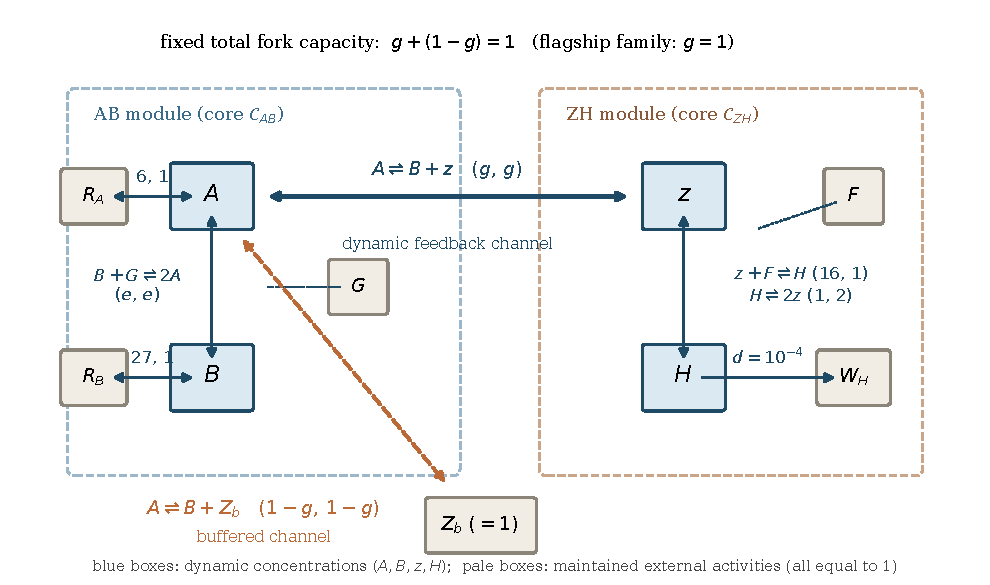
\includegraphics[width=.96\linewidth]{figures/network.pdf}
\caption{Reaction architecture and the controlled intervention. Blue boxes are dynamic concentrations, pale boxes maintained external activities. The fork $A\rightleftharpoons B+z$ is the only reaction shared by the two modules. In the routed family its capacity is split between the dynamic channel (coefficients $g,g$) whose product $z$ enters the $ZH$ module and a buffered channel $A\rightleftharpoons B+Z_b$ (coefficients $1-g,1-g$, $Z_b\equiv1$) whose product is held fixed; the total forward and reverse capacity $g+(1-g)=1$ is the invariant of the intervention. The flagship family is $g=1$. The output $H\to W_H$ is an ideal irreversible sink until Section~\ref{sec:persistence}.}\label{fig:network}
\end{figure}

\subsection{The two distinguished cores and their activity}\label{sec:cores}

Restricting channels 1 and 6 to the species $(A,B)$, with $z$ external, and channels 2 and 3 to $(z,H)$, both restrictions have the oriented stoichiometric matrix
\[
S_c=\begin{pmatrix}-1&2\\1&-1\end{pmatrix}.
\]
For oriented net currents $(j,k)$ of the two channels, the production vector is $S_c(j,k)^{\mathsf T}=(-j+2k,\,j-k)$, and we say the core is \emph{strictly productive} at a state if both components are positive; this forces $j,k>0$ and is feasible (take $(j,k)=(3,2)$). Deleting either channel makes strict production of both species impossible even for signed currents, and a proper nonempty species restriction cannot remain autonomous, since one remaining channel loses its reactant or its product. Thus $\cAB$ and $\cZH$ are minimal gain-two autocatalytic cores in the sense of~\cite{blokhuis2020,nandan2026}. We do not claim that they exhaust the cores of the network; every statement below concerns these two distinguished cores.

\begin{definition}[Actual production and activity signature]\label{def:activity}
At a state $x$ of the flagship system put $j=A-Bz$, $k=e(B-A^2)$, $\ell=16z-H$, $m=H-2z^2$ and
\begin{equation}\label{eq:production}
p_{AB}(x)=(p_{AB,A},p_{AB,B})=(-j+2k,\;j-k),\qquad
p_{ZH}(x)=(p_{ZH,z},p_{ZH,H})=(-\ell+2m,\;\ell-m).
\end{equation}
The \emph{activity signature} of $x$ is the pair of truth values ($\cAB$ strictly productive at $x$, $\cZH$ strictly productive at $x$). The \emph{eventual} signature of a trajectory is the signature that holds for all sufficiently large times, when it exists.
\end{definition}

These are deterministic identities in the actual net currents at the state; no stochastic process is involved. Direct cancellation gives, at every state and for all rates,
\begin{equation}\label{eq:balance-identity}
p_{AB,A}+2\,p_{AB,B}+p_{ZH,z}=F_z,
\end{equation}
because $-j+2k+2(j-k)=j$ and $-\ell+2m=-uz+H+2H-2vz^2$ with $u=16,v=2$. At a stationary state the right side vanishes, so the two cores cannot both be strictly productive there (Section~\ref{sec:activity}).

\subsection{Clamped modules and the routed fork}\label{sec:clamp}

\begin{definition}[Clamping]
Clamping a module means fixing the complementary dynamic concentrations in the full equations~\eqref{eq:general} while retaining every reservoir and every constant input or linear load induced by the other reactions. For the $AB$ module fix $z>0$ and consider $(F_A,F_B)$ as equations in $(A,B)$; for the $ZH$ module fix $A,B>0$ and consider $(F_z,F_H)$ as equations in $(z,H)$. Clamping is an equilibrium calculation used for comparison; it neither deletes boundary terms nor retunes rates.
\end{definition}

\begin{definition}[Routed feedback intervention]
Split channel~1 into two channels of identical stoichiometry,
\begin{equation}\label{eq:routing}
A\rightleftharpoons B+z\ \ (g,g),\qquad A\rightleftharpoons B+Z_b\ \ (1-g,1-g),\qquad Z_b\equiv1,\qquad 0\le g\le1 .
\end{equation}
The \emph{fixed total fork capacity} is the invariant $g+(1-g)=1$ of both the forward and the reverse coefficient sums. With $c_g(z)=1-g+gz$ and $j_g=g(A-Bz)$ the routed equations at the flagship rates are
\begin{equation}\label{eq:routed}
\begin{aligned}
\dot A&=6-2A+c_g(z)B+2e(B-A^2),& \dot B&=27+A-(1+c_g(z))B-e(B-A^2),\\
\dot z&=j_g-16z-4z^2+3H,& \dot H&=16z+2z^2-(2+d)H.
\end{aligned}
\end{equation}
\end{definition}

Equation~\eqref{eq:ode} is $g=1$. At $g=0$ the $z$ and $H$ equations no longer contain $A,B$ and the $A,B$ equations no longer contain $z$: the modules are decoupled, each running with its own reservoirs and loads, and the buffered fork is the isolated $AB$ module's version of channel~1. The invariant of the intervention is the stipulated capacity; it is not a claim of fixed energy dissipation, fixed material throughput, or equal realized fork flux at every state. The routed domain used below is
\begin{equation}\label{eq:domains}
\Rr=\Bigl(\tfrac{999}{10^8},\tfrac{1001}{10^8}\Bigr)\times\Bigl(\tfrac{999999}{10^6},1\Bigr)\ni(e,g).
\end{equation}

\subsection{A common mass-balanced realization}\label{sec:thermo}

Assign masses $(2,1,1,2,1)$ to $(A,B,z,H,Z_b)$ and $(1,3,2,1,2)$ to $(F,G,R_A,R_B,W_H)$. Every reaction of Table~\ref{tab:reactions}, in its completed form with external species, conserves this mass. In units $RT=1$ assign standard chemical potentials
\begin{equation}\label{eq:mu}
(\mu_A,\mu_B,\mu_z,\mu_H,\mu_{Z_b})=(0,0,0,-\log2,0),\qquad(\mu_F,\mu_G,\mu_{R_A},\mu_{R_B})=(\log8,0,\log6,\log27).
\end{equation}
Then $k_+/k_-=\exp(\sum\mu_{\mathrm{reactant}}-\sum\mu_{\mathrm{product}})$ for every reversible pair at the flagship rates: the ratios are $1,16,1/2,6,27,1$ for channels $1$--$6$ and $1$ for the buffered fork. Positive common kinetic prefactors then realize the individual rate coefficients. The ideal sink is explicitly excluded from this finite-potential relation until Section~\ref{sec:persistence}; the system is driven by maintained buffers and is not detailed balanced.

\subsection{Principal results}\label{sec:results}

Write $\Phi_t(x)$ for the unique positive solution of~\eqref{eq:ode} with $\Phi_0(x)=x$ and $\B_s=\{x\in D:\Phi_t(x)\to s\}$ for the basin of an equilibrium $s$.

\begin{theorem}[Global selection in the flagship family]\label{thm:G}
Let $e\in I$. Every positive initial state has a unique global positive solution of~\eqref{eq:ode}, and every such solution converges to an equilibrium. There are exactly three positive equilibria $s_-,s_0,s_+$, ordered by their $z$ coordinates, which lie respectively in $(0.9,1.1)$, $(1.9,2.1)$ and $(2.9,3.1)$; all three are nondegenerate. The outer equilibria are hyperbolic sinks with four real negative eigenvalues; the middle equilibrium has three real negative eigenvalues and one positive real eigenvalue. The sink basins are nonempty, open and disjoint, and
\begin{equation}\label{eq:boundary}
\partial\B_{s_-}\cap D=\partial\B_{s_+}\cap D=\B_{s_0}=:W .
\end{equation}
$W$ is an embedded real-analytic hypersurface of $D$, and both branches of the local unstable curve of $s_0$ lie in $D$ and converge forward to opposite sinks. In the absorbing region $\Omega$ of~\eqref{eq:Omega}, the strict inequalities $V(x)<V(s_0)$ and $B(x)>B(s_0)$ imply $x\in\B_{s_-}$, and $V(x)<V(s_0)$ with $B(x)<B(s_0)$ imply $x\in\B_{s_+}$, where $V$ is the response potential~\eqref{eq:V}.
\end{theorem}

\begin{theorem}[Feedback-induced coexistence in the routed family]\label{thm:C}
Let $e>0$. Both clamped modules have exactly one positive equilibrium for every positive clamped input. For $e\le1/50000$ the isolated system ($g=0$) and every weak-feedback system with $g\in[1/100,1/10]$ have exactly one positive equilibrium. For $(e,g)\in\Rr$ the routed system~\eqref{eq:routed} has two distinct positive equilibria, with $z$ coordinates in $(0.9957,0.9959)$ and $(2.9762,2.9766)$, each locally exponentially attracting: there is an explicit quadratic form $E$ and a box around each equilibrium on which every forward solution stays, satisfies $E(t)\le E(0)e^{-t/100}$, and converges to that equilibrium. Distinct $(e,g)$ give distinct vector fields. The theorem asserts local attracting coexistence on $\Rr$; it does not assert global convergence or an exact equilibrium count there.
\end{theorem}

\begin{theorem}[Eventual activity and its information limit]\label{thm:A}
Let $e\in I$. Every positive solution of~\eqref{eq:ode} eventually has $\cAB$ inactive and $\cZH$ strictly productive; more precisely, for all sufficiently large $t$,
\begin{equation}\label{eq:margins}
p_{AB,B}<-3,\qquad p_{ZH,z}>2,\qquad p_{ZH,H}>\tfrac1{4000}.
\end{equation}
Both sinks $s_-$ and $s_+$ have this signature while every one of their four concentrations differs. If on an interval $[a,b]$ all of $p_{AB,A},p_{AB,B},p_{ZH,z}$ are at least $\eta>0$ and $z(b)\le12$, then $b-a\le3/\eta$.
\end{theorem}

Theorem~\ref{thm:G} and the activity assertions of Theorem~\ref{thm:A} are proved in Sections~\ref{sec:global} and~\ref{sec:activity} and compiled as the Lean structures \lean{FlagshipGResolution} and \lean{FlagshipAResolution}; Theorem~\ref{thm:C} is proved in Sections~\ref{sec:stationary}--\ref{sec:feedback} and compiled as the structure \lean{RoutedCResolution} on the region \lean{routedBistableRegion} of Appendix~\ref{app:verification}. The fold theorem (Theorem~\ref{thm:fold}) and the consequences of Section~\ref{sec:consequences} are conventional. Table~\ref{tab:scope} summarizes the families and the evidence.

\begin{table}[tb]\centering\small
\begin{tabular}{@{}>{\raggedright\arraybackslash}p{.28\linewidth}>{\raggedright\arraybackslash}p{.30\linewidth}>{\raggedright\arraybackslash}p{.36\linewidth}@{}}\toprule
Result & Family and domain & Evidence\\\midrule
Clamped-module uniqueness (Prop.~\ref{prop:clamped}) & all positive rates, any clamped input & conventional; Lean (\lean{CoreCouplingCAC})\\
Unistationarity for $d\ge1$ (Prop.~\ref{prop:preservation}) & all positive rates with $d\ge1$ & conventional; Lean\\
Isolated and weak uniqueness (Prop.~\ref{prop:weak}) & routed, $g\in\{0\}\cup[1/100,1/10]$, $0<e\le1/50000$ & conventional; Lean\\
Exactly three equilibria, spectra (Thm.~\ref{thm:count}) & flagship, $e\in I$ & Descartes/Bernstein rational certificates; Lean\\
Two attracting equilibria (Thm.~\ref{thm:C}) & routed, $(e,g)\in\Rr$ & rational contraction certificate; Lean\\
Saddle-node (Thm.~\ref{thm:fold}) & routed path $e=10^{-5}$, $g\in[0.1,1-5\cdot10^{-7}]$ & exact rational interval certificate + conventional\\
Global convergence, basin geometry, selection rule (Thm.~\ref{thm:G}) & flagship, all of $D$ & conventional proof; Lean\\
Measure zero, eventual test, budget (Sec.~\ref{sec:consequences}) & flagship & conventional\\
Eventual activity (Thm.~\ref{thm:A}) & flagship & conventional; Lean\\
Local persistence, reversible sink (Sec.~\ref{sec:persistence}) & neighbourhoods of the flagship sinks & conventional\\\bottomrule
\end{tabular}
\caption{Scope of the results. ``Lean'' means a compiled declaration listed in Appendix~\ref{app:verification}; ``conventional'' means a proof given in this paper.}\label{tab:scope}
\end{table}

\section{Stationary responses: clamped uniqueness, exact reconstruction, and the load mechanism}\label{sec:stationary}

\subsection{Each clamped module has one positive equilibrium}

\begin{proposition}\label{prop:clamped}
For all positive rates and every clamped $z>0$, the clamped $AB$ module has exactly one positive equilibrium; for every clamped $A>0$ and $B>0$, the clamped $ZH$ module has exactly one positive equilibrium.
\end{proposition}
\begin{proof}
For $AB$, solve $F_B=0$ for $B=(b+A+eA^2)/(1+z+e)$ and substitute into $F_A=0$:
\begin{equation}\label{eq:ABquad}
e(2+z)A^2+(2+z)A-\bigl[a(1+z+e)+(z+2e)b\bigr]=0 .
\end{equation}
The left side is strictly increasing on $A>0$, negative at $A=0$ and unbounded, so it has exactly one positive root, and the reconstructed $B$ is positive. For $ZH$, eliminate $H=(uz+vz^2)/(2+d)$ from $F_H=0$ and substitute into $F_z=0$:
\begin{equation}\label{eq:ZHquad}
v(1+2d)z^2+\bigl[(2+d)B-u(1-d)\bigr]z-(2+d)A=0 .
\end{equation}
The leading coefficient is positive and the constant term negative, so the two real roots have opposite signs and exactly one is positive; $H$ is then positive and unique. Both arguments are uniform in the clamped inputs and in the sign of the linear coefficient of~\eqref{eq:ZHquad}.
\end{proof}

\subsection{Exact reconstruction and the unistationary regime}\label{sec:reconstruction}

Put $c_0=a+2b$ and define, for $z>0$,
\begin{equation}\label{eq:reconstruction}
\begin{gathered}
B_p(z)=\frac{c_0}{z+2},\qquad K_p(z)=\frac{v(1+2d)z^2-u(1-d)z}{2+d},\\
A_p(z)=zB_p(z)+K_p(z),\qquad H_p(z)=\frac{uz+vz^2}{2+d},
\end{gathered}
\end{equation}
and the scalar residual
\begin{equation}\label{eq:E}
E_p(z)=b-(1+e)B_p(z)+K_p(z)+eA_p(z)^2 .
\end{equation}
The combinations $F_A+2F_B=c_0-(z+2)B$ and $(2+d)F_z+3F_H=(2+d)\bigl(A-Bz-K_p(z)\bigr)$ show that every equilibrium has $B=B_p(z)$, $A=A_p(z)$, $H=H_p(z)$; writing $\ell_p(z)=(A_p,B_p,z,H_p)(z)$, direct substitution gives the stronger identity
\begin{equation}\label{eq:field-identity}
F\bigl(\ell_p(z)\bigr)=\bigl(-2E_p(z),\,E_p(z),\,0,\,0\bigr).
\end{equation}
Hence positive equilibria correspond bijectively to zeros $z>0$ of $E_p$ with $A_p(z)>0$; $B_p$ and $H_p$ are automatically positive. The positivity qualification is essential and is not implied by the rational reduction. We stress that $E_p$ is a stationary residual, not the $z$ component of the dynamics away from equilibrium.

\begin{proposition}[Unistationarity when the loss rate is at least the reference rate]\label{prop:preservation}
For all positive rates with $d\ge1$ the full system~\eqref{eq:general} has exactly one positive equilibrium.
\end{proposition}
\begin{proof}
If $d\ge1$ then $K_p$ is nonnegative and strictly increasing on $z>0$, $B_p$ is strictly decreasing, and $zB_p=c_0-2B_p$ is strictly increasing; hence $A_p>0$ is strictly increasing, and each varying term of $E_p$, namely $-(1+e)B_p$, $K_p$ and $eA_p^2$, is strictly increasing. So $E_p$ is strictly increasing on $(0,\infty)$. Moreover $E_p(0)=-a/2-e(a+2b)/2<0$, and for $R=1+(1+e)c_0/b$ one has $E_p(R)\ge b-(1+e)c_0/(R+2)>0$. Continuity gives a root in $(0,R)$, monotonicity gives uniqueness, and the reconstruction is positive.
\end{proof}

The mechanism that permits multiplicity for $d<1$ is visible in~\eqref{eq:reconstruction}: the load $K_p$ then contains the negative linear term $-u(1-d)z/(2+d)$, so neither $K_p$ nor $E_p$ need be monotone. The threshold $d=1$ is relative to the unit reverse rate of channel~2; it is not a universal degradation threshold.

\subsection{Routed balances, the load mechanism, and weak-feedback uniqueness}

At every stationary state of the routed system~\eqref{eq:routed}, adding the $A$ and $B$ equations once and twice, and combining the $z$ and $H$ equations, gives
\begin{equation}\label{eq:balance}
D_g(z)\,B=60,\qquad eA^2+A+(1-e)B=33,\qquad g(A-Bz)=k(z),\qquad H=\frac{16z+2z^2}{2+d},
\end{equation}
where
\begin{equation}\label{eq:Dk}
D_g(z)=3-g+gz,\qquad k(z)=\frac{20004\,z^2-159984\,z}{20001}=K_p(z)\big|_{(u,v,d)=(16,2,10^{-4})}.
\end{equation}
For $0<g\le1$ and $z>0$ all denominators are positive. Define
\begin{equation}\label{eq:Q}
B_g(z)=\frac{60}{D_g(z)},\qquad A_g(z)=zB_g(z)+\frac{k(z)}{g},\qquad Q_e(z,g)=eA_g(z)^2+A_g(z)+(1-e)B_g(z)-33 .
\end{equation}
Positive stationary states of~\eqref{eq:routed} correspond exactly to roots $z>0$ of $Q_e(\cdot,g)$ with $A_g(z)>0$, all coordinates being reconstructed by~\eqref{eq:balance}; at $g=1$ this is~\eqref{eq:reconstruction} with $Q_e(z,1)=E_p(z)$ at the flagship rates. As before the routed field satisfies $F\bigl(A_g,B_g,z,H_g\bigr)=Q_e\,(-2,1,0,0)$.

\begin{lemma}[Multiplicity requires a decreasing load secant]\label{lem:load}
Let $0<g\le1$ and let $x,y$ be positive stationary states of~\eqref{eq:routed} with $z_y>z_x$. Then $\Delta B:=B_x-B_y>0$, $0<A_y-A_x\le\Delta B$, and
\begin{equation}\label{eq:load}
k(z_y)-k(z_x)=g(A_y-A_x)-(3-g)\Delta B\le(2g-3)\Delta B<0 .
\end{equation}
Consequently, on any interval of $z$ on which $k$ is nondecreasing there is at most one positive stationary state.
\end{lemma}
\begin{proof}
$B=60/D_g(z)$ is strictly decreasing in $z$, so $\Delta B>0$. Subtracting the second balance of~\eqref{eq:balance} at the two states gives $(A_y-A_x)\{1+e(A_y+A_x)\}=(1-e)\Delta B$, hence $0<A_y-A_x\le\Delta B$. From $gzB=60-(3-g)B$ the third balance reads $k(z)=gA-60+(3-g)B$, and subtracting gives~\eqref{eq:load}.
\end{proof}

\begin{proposition}[Isolated and weak-feedback uniqueness]\label{prop:weak}
Let $0<e\le1/50000$. At $g=0$ and for every $g\in[1/100,1/10]$ the routed system has exactly one positive equilibrium, and it is nondegenerate.
\end{proposition}
\begin{proof}
At $g=0$ the $AB$ balance gives $B=20$ and $eA^2+A=13+20e$, with a unique positive $A$; the $ZH$ equations give $16z+2z^2=(2+d)H$ and $k(z)=0$, whose positive solution is $z=159984/20004$, followed by $H$. For $g\in[1/100,1/10]$ we first show $z>4$ at every positive stationary state. If $z\le4$ then $D_g(z)\le3+3g\le3.3$, so $B\ge200/11$; the second balance then gives $A<33-(1-e)B<15$, and $B<34$. For $0<z\le4$ one has $k(z)\le-3.99\,z$, so $gA=gBz+k(z)\le(3.4-3.99)z<0$, contradicting $A>0$. On $z>4$ the load satisfies $k'(z)=(40008z-159984)/20001>0$, so Lemma~\ref{lem:load} gives at most one state. Existence: the same estimate shows $A_g<0$ on $(0,4]$, and on $z>4$ the function $A_g$ is strictly increasing, since differentiating $D_gB_g=60$ gives $B_g+zB_g'=-(3-g)B_g'/g$ and hence $A_g'=-(3-g)B_g'/g+k'/g>0$; as $A_g\to+\infty$, it has exactly one zero $z_1>4$. There $Q_e(z_1,g)=(1-e)B_g(z_1)-33<0$ because $z_1>4$ gives $B_g<20$, while $Q_e\to+\infty$ as $z\to\infty$; so a root with $A_g>0$ exists in $(z_1,\infty)$, and every positive stationary state lies there. Nondegeneracy: at such a state,
\[
Q_z=\{1+2eA_g\}A_g'+(1-e)B_g'\ \ge\ A_g'+(1-e)B_g'\ \ge\ -B_g'\Bigl[\frac{3-g}{g}-(1-e)\Bigr]>0,
\]
since $-B_g'>0$ and $(3-g)/g\ge29$. The determinant identity~\eqref{eq:det} then makes the stationary Jacobian nonsingular.
\end{proof}

\subsection{Exactly three flagship equilibria and their spectra}

\begin{theorem}\label{thm:count}
For every $e\in I$ the flagship system~\eqref{eq:ode} has exactly three positive equilibria $s_-,s_0,s_+$, with $z$ coordinates in $(0.9,1.1)$, $(1.9,2.1)$ and $(2.9,3.1)$. Each is a simple root of $E_p$, hence a nondegenerate equilibrium. The Jacobian at $s_\pm$ has four distinct real eigenvalues in $(-80,-10)$, $(-10,-2)$, $(-2,-1/2)$, $(-1/2,0)$; at $s_0$ the first three intervals are the same and the fourth eigenvalue lies in $(0,1/10)$.
\end{theorem}
\begin{proof}
\emph{Positivity and brackets.} At the flagship rates $c_0=60$, $B(z)=60/(z+2)$ and $K(z)=\beta z^2-\alpha z$ with $\beta=6668/6667$, $\alpha=53328/6667$. For $0<z\le4$, $B\ge10$ and $K\ge-8z$, so $A(z)\ge2z>0$: the reconstruction is positive on every bracket used below. Exact rational substitution gives the signs $-,+,+,-,-,+$ of $E_e$ at $z=0.9,1.1,1.9,2.1,2.9,3.1$ at both endpoints of $I$; since $A,B,K$ do not depend on $e$, $E_e(z)$ is affine in $e$ and the signs persist on $I$. The intermediate value theorem supplies a root in each of the three brackets.

\emph{Exactly three roots, all simple.} Clearing the denominator, $Q_e(z):=(z+2)^2E_e(z)$ is a polynomial of degree six; explicitly, up to a positive constant factor,
\begin{equation}\label{eq:P}
\begin{aligned}
P_e(z)={}&44462224\,e\,z^6-533333312\,e\,z^5+(5511662368\,e+44455556)z^4\\
&-(23464426176\,e+177715552)z^3+(86062436496\,e-44208877)z^2\\
&+(711395568-2666933340\,e)z-5333866680\,e-533386668 .
\end{aligned}
\end{equation}
The substitution $z=8t/(1+t)$ maps $t>0$ bijectively onto $0<z<8$, and $\widetilde P_e(t)=6667^2(1+t)^6Q_e(8t/(1+t))=\sum_{i=0}^6(C_i+D_ie)t^i$ has the integer coefficients listed in Table~\ref{tab:descartes}. At both endpoints of $I$, hence throughout $I$ by affine dependence, the ascending coefficient signs are $(-,+,+,-,-,+,+)$: exactly three sign changes. By Descartes' rule $\widetilde P_e$ has at most three positive roots counted with multiplicity, and the three bracketed roots exhaust them and are simple. The M\"obius substitution has positive derivative, so simplicity transfers to $E_e$ on $(0,8)$. For $z\ge8$, $\beta z-\alpha>0$ gives $K>0$ while $B\le6$, so $E_e\ge27-6(1+e)>0$. Hence there are exactly three positive equilibria. (A second, derivative-based route: $P_e''(0)<-8.4\cdot10^7$ and $P_e^{(4)}>10^9$ on $[0,12]$ by exact interval evaluation, so $P_e''$ is convex and has at most one positive zero and Rolle's theorem bounds the positive zeros of $P_e$ on $[0,12]$ by three; positive stationary states have $z<12$ because $A<33$ while $k(z)>33$ for $z\ge12$.)

\emph{Nondegeneracy.} Ordering the variables as $(B,A,H,z)$ and the equations as $F_A+2F_B$, $(2+d)F_z+3F_H$, $F_H$, $F_B$, the first three equations have a triangular derivative block with diagonal $-(z+2)$, $2+d$, $-(2+d)$, and the Schur complement of the fourth is the derivative of $F_B$ along the reconstruction. Including the transformation determinant $2+d$ and the positive sign of the permutation,
\begin{equation}\label{eq:det}
\det J_F\bigl(\ell_p(z)\bigr)=(z+2)(2+d)\,E_p'(z),
\end{equation}
and, for the routed field with $g>0$, $\det J=g(2+d)D_g(z)\,\partial_zQ_e$. Simple roots are therefore nondegenerate equilibria, and since $E_e(0)<0$ the derivative signs at the ordered roots are $+,-,+$.

\emph{Spectra.} At $g=1$ the physical Jacobian is
\begin{equation}\label{eq:J}
J=\begin{pmatrix}
-2-4eA&z+2e&B&0\\ 1+2eA&-1-z-e&-B&0\\ 1&-z&-B-16-8z&3\\ 0&0&16+4z&-2-d
\end{pmatrix}.
\end{equation}
Substitute $B=60/(z+2)$, treat $e\in[0,1/50000]$ and $q:=eA\in[0,34/50000]$ as independent parameters (at a stationary state $A<33$), and multiply $\det(\lambda I-J)$ by $z+2$; the result is a cubic in $z$ whose coefficients are affine in $(e,q)$. At $\lambda=-80,-10,-2,-1/2,1/10$ its sign on each of the three $z$ brackets, uniformly in $(e,q)$, is $+,-,+,-,+$; at $\lambda=0$ the sign is $+,-,+$ on the three brackets respectively. Each sign is certified by the positivity of all degree-three Bernstein coefficients of the appropriately signed cubic on the bracket, evaluated at the four $(e,q)$ corners, with uniform lower bounds $48{,}008{,}578$; $69{,}321$; $153$; $63$; $55$ for the five $\lambda$ tests and $8$; $7$; $14$ for the three zero tests (Appendix~\ref{app:cert}). A monic quartic with these sign alternations has four distinct real roots, one in each of $(-80,-10)$, $(-10,-2)$, $(-2,-1/2)$, and a fourth in $(-1/2,0)$ at the outer states or in $(0,1/10)$ at the middle state.
\end{proof}

\begin{remark}
The local stability assertions are derived from the displayed Jacobian and rational sign certificates; no stability label is imported from the verbal description of the source example in~\cite{nandan2026}, whose network differs from ours by the reverse channel and the sink.
\end{remark}

\section{Feedback creates stable alternatives: the routed family}\label{sec:feedback}

\subsection{Rational contraction certificates and Theorem~\ref{thm:C}}

Both stability certificates in this paper use one elementary device. Let $y=Tx=(A+B,-B,z,H)$; in these coordinates the routed vector field $G=TFT^{-1}$ is quadratic with Jacobian
\begin{equation}\label{eq:Jr}
J_r(y)=\begin{pmatrix}
-1-2eA&-e(1+2A)&0&0\\
-1-2eA&-3+g-gz-e-2eA&gB&0\\
g&g(1+z)&-gB-16-8z&3\\
0&0&16+4z&-2-d
\end{pmatrix},
\end{equation}
where $A=y_1+y_2$ and $B=-y_2$.

\begin{lemma}[Comparison-energy certificate]\label{lem:certificate}
Let $X$ be a convex box of states containing an equilibrium $c$, and let $M$ be a constant matrix with $(J_r)_{ii}(y)\le M_{ii}$ and $|(J_r)_{ij}(y)|\le M_{ij}$ $(i\ne j)$ for all $y\in TX$. Suppose positive vectors $l,r\in\R^4$ satisfy
\begin{equation}\label{eq:row}
l_i(Mr)_i+r_i(M^{\mathsf T}l)_i\le-\kappa\,l_ir_i\qquad(i=1,\dots,4)
\end{equation}
for some $\kappa>0$. Then $E(y)=\sum_i(l_i/r_i)\bigl(y_i-(Tc)_i\bigr)^2$ satisfies $\dot E\le-\kappa E$ along solutions in $X$. Consequently every sufficiently small sublevel set of $E$ contained in $X$ is forward invariant, solutions starting there exist for all time, remain in the sublevel, converge to $c$, and satisfy $E(t)\le E(0)e^{-\kappa t}$.
\end{lemma}
\begin{proof}
Because $G$ is quadratic its exact secant is $G(y)-G(Tc)=J_r\bigl(\tfrac{y+Tc}{2}\bigr)(y-Tc)$, and the midpoint lies in $TX$ by convexity. Put $w_i=(y_i-(Tc)_i)/r_i$. Bounding only the off-diagonal terms by absolute values and using $2|w_iw_j|\le w_i^2+w_j^2$ while keeping the signed diagonal terms gives
\[
\dot E\le\sum_i\bigl[l_i(Mr)_i+r_i(M^{\mathsf T}l)_i\bigr]w_i^2\le-\kappa E .
\]
On the boundary of a sublevel set inside $X$ the derivative is at most $-\kappa E<0$, so the sublevel is forward invariant, and Gr\"onwall gives the decay. Global existence follows by extending the polynomial field with a smooth cutoff that equals one on a large ball containing $X$; the extended field is bounded and globally Lipschitz, its solutions from the sublevel never leave the region where the cutoff is one, and by local uniqueness every forward solution of the original polynomial field coincides with the constructed one.
\end{proof}

The argument estimates the full four-dimensional nonlinear field on a box; it does not identify the stationary elimination $Q_e$ with a scalar differential equation.

\begin{proof}[Proof of Theorem~\ref{thm:C}]
Clamped uniqueness is Proposition~\ref{prop:clamped}; isolated and weak uniqueness is Proposition~\ref{prop:weak}. Injectivity of the family: at the fixed positive state $(A,B,z,H)=(1,2,1,8)$ the routed field gives $\dot A+\dot B=30+e$ and $\dot z=4-g$, so $(e,g)$ is recovered from the vector field. For coexistence, on the closure of $\Rr$ exact rational sign tests of the numerator of $Q_e$ (Bernstein conversion in $g$ of degree four and endpoints in $e$, Appendix~\ref{app:cert}) isolate roots with
\[
0.9957<z_-<0.9959,\qquad 2.9762<z_+<2.9766,
\]
and the reconstructed states lie strictly inside the boxes
\begin{align*}
L_-&=(12.96,\,20.02,\,0.9956,\,8.94),&U_-&=(12.99,\,20.04,\,0.996,\,8.98),\\
L_+&=(20.92,\,12.05,\,2.9761,\,32.64),&U_+&=(20.96,\,12.07,\,2.9767,\,32.70).
\end{align*}
Let $M_\pm$ bound~\eqref{eq:Jr} on these boxes over the closed parameter rectangle, entry by entry as in Lemma~\ref{lem:certificate}. The positive rational weights $l,r$ of Table~\ref{tab:weights} satisfy~\eqref{eq:row} with $\kappa=1/100$; every acceptance comparison is an inequality between fractions. Lemma~\ref{lem:certificate} gives, for each of the two disjoint boxes, an invariant sublevel set on which every forward solution converges exponentially to the equilibrium in that box. The two equilibria are distinct since their $z$ brackets are disjoint.
\end{proof}

\begin{remark}[Quantitative neighbourhoods at $g=1$]\label{rem:cac}
The same boxes, comparison matrices and weights certify the flagship sinks at $e=10^{-5}$, $g=1$, where the outer roots lie in $[0.995794,0.995795]$ and $[2.976367,2.976368]$. With $\rho=10^{-12}$ the sublevel $\{E\le\rho\}$ is contained in the expanded positive box of Table~\ref{tab:cacboxes}, and it contains the cube $U_c=\{x:|(Tx)_i-(Tc)_i|\le10^{-8}\}$ because $1/4\le l_i/r_i\le100$. Every forward solution from $U_c$ therefore remains positive, converges to $c$, satisfies $E(t)\le E(0)e^{-t/100}$, hence $|A(t)-c_A|\le4\sqrt{E(0)}e^{-t/200}$ and $|B-c_B|,|z-c_z|,|H-c_H|\le2\sqrt{E(0)}e^{-t/200}$, and keeps both $\cZH$ production margins at least $10^{-4}$ throughout the box. This local statement is compiled as \lean{CoreCouplingCAC.coreCouplingCACResolution}; Theorem~\ref{thm:G} supersedes it qualitatively but not quantitatively.
\end{remark}

\subsection{A certified saddle-node on the routed path}\label{sec:fold}

Fix $e=10^{-5}$ and consider $g\in[1/10,1999999/2000000]$. Positive stationary states are uniformly confined: by~\eqref{eq:balance}, $A<33$ and $B<34$, and $k(z)\le A<33$ forces $z<12$; hence $D_g<15$ and $B>4$; the $A$ equation gives $A\ge6/(2+66e)>2.9$; if $z<1$ then $k(z)<0$, so $gA<gBz$ and $z>A/B>2.9/34>0.08$; finally $H=(16z+2z^2)/(2+d)\in(0.5,240)$. These bounds hold on the whole segment and exclude escape to the concentration boundary. If every stationary Jacobian on this segment were nonsingular, the implicit function theorem and properness would make the number of positive stationary states constant along the connected segment. But exact Sturm isolation of the cleared polynomial gives one positive reconstructed root at $g=1/10$ and three at $g=1999999/2000000$, both polynomials being square-free (Appendix~\ref{app:fold}), and by~\eqref{eq:det} nonsingularity is equivalent to simplicity. Hence some interior positive equilibrium is singular. The following theorem locates one such transition.

\begin{theorem}[Certified local saddle-node]\label{thm:fold}
For $e=10^{-5}$ there is a unique solution $(z_*,g_*)$ of $Q_e=\partial_zQ_e=0$ in the rational box
\begin{equation}\label{eq:foldbox}
|z-1.617456101591|\le10^{-9},\qquad|g-0.970187992295|\le10^{-10}.
\end{equation}
There $\partial_gQ_e>0$, $\partial_{zz}Q_e<0$, all reconstructed concentrations are positive, and the full Jacobian has a simple zero eigenvalue and three eigenvalues with negative real parts. The equilibrium undergoes a nondegenerate saddle-node: a sink--saddle pair exists locally for $g>g_*$ and no local pair exists for $g<g_*$; the lower-$z$ member of the pair is the sink. No uniqueness of the fold outside this box and no complete bifurcation diagram is asserted.
\end{theorem}
\begin{proof}
Let $f=(Q_e,\partial_zQ_e)$ as a function of $(z,g)$, let $c$ be the rational centre of~\eqref{eq:foldbox} and $r=(10^{-9},10^{-10})$ its radii, and let $C=Df(c)^{-1}$ (an exact rational matrix). Rational interval evaluation on the box $X=c+[-r,r]$ gives
\[
\|I-C\,Df(X)\|_r<1.10\cdot10^{-7}<1,\qquad\bigl|-Cf(c)+(I-C\,Df(X))[-r,r]\bigr|<r
\]
componentwise, where $\|\cdot\|_r$ is the radius-weighted maximum norm. Thus $x\mapsto x-Cf(x)$ maps the closed box strictly into its interior and is a contraction there, so Banach's theorem gives existence and uniqueness of the zero~\cite{moore1977,rump1983}. On the same box, $3.48109471<\partial_gQ_e<3.48109479$ and $-0.58505657<\partial_{zz}Q_e<-0.58505652$; the reconstruction is positive, with $A\simeq16.3264$, $B\simeq16.6711$, $H\simeq15.5550$.

The routed field satisfies $F(A_g,B_g,z,H_g)=Q_e\,(-2,1,0,0)$ on the reconstructed curve and $\det J=g(2+d)D_g\,\partial_zQ_e$, so $J$ is singular at the certified point. Its characteristic polynomial is $\lambda(\lambda^3+c_1\lambda^2+c_2\lambda+c_3)$ with $51.71353<c_1<51.71354$, $202.05986<c_2<202.05988$, $151.36638<c_3<151.36640$; since $c_i>0$ and $c_1c_2>c_3$ the cubic factor is Hurwitz~\cite{gantmacher1959} and the zero eigenvalue is simple.

For the dynamical nondegeneracy conditions~\cite{sotomayor1973,kuznetsov2004}, let $v=\partial_z(A_g,B_g,z,H_g)$, a nonzero kernel vector at the fold, and let $w$ be a left null vector of $J$. We claim $w\cdot(-2,1,0,0)\ne0$. Let $T$ be the invertible linear map sending $F$ to the balances $G=(F_A+2F_B,\,(2+d)F_z+3F_H,\,F_H,\,F_B)$; then $T(-2,1,0,0)=(0,0,0,1)$, and the derivative of $(G_1,G_2,G_3)=(60-D_gB,\,(2+d)(g(A-Bz)-k(z)),\,16z+2z^2-(2+d)H)$ with respect to $(B,A,H)$ is triangular with diagonal $-D_g$, $(2+d)g$, $-(2+d)$, hence invertible. So the first three rows of $DG=TJ$ are independent, and since $\operatorname{rank}J=3$ every left null vector $w'=T^{-\mathsf T}w$ of $DG$ has $w'_4\ne0$; therefore $w\cdot(-2,1,0,0)=w'\cdot T(-2,1,0,0)=w'_4\ne0$. Differentiating the field identity once in $g$ and twice in $z$ along the curve, all terms containing $J$ vanish after multiplication by $w$, leaving
\[
w\cdot f_g=\partial_gQ_e\;w\cdot(-2,1,0,0)\ne0,\qquad w\cdot D^2_xf[v,v]=\partial_{zz}Q_e\;w\cdot(-2,1,0,0)\ne0 .
\]
Equivalently the parameterized scalar Morse lemma gives $g-g_*=\bigl(-\partial_{zz}Q_e/(2\partial_gQ_e)\bigr)(z-z_*)^2+o((z-z_*)^2)$ with positive coefficient, so the pair exists for $g>g_*$. Three eigenvalues remain negative nearby. On the lower-$z$ branch $\partial_zQ_e>0$, so by the determinant identity and the Hurwitz cubic the small fourth eigenvalue is negative; on the upper branch it is positive.
\end{proof}

\begin{figure}[tb]\centering
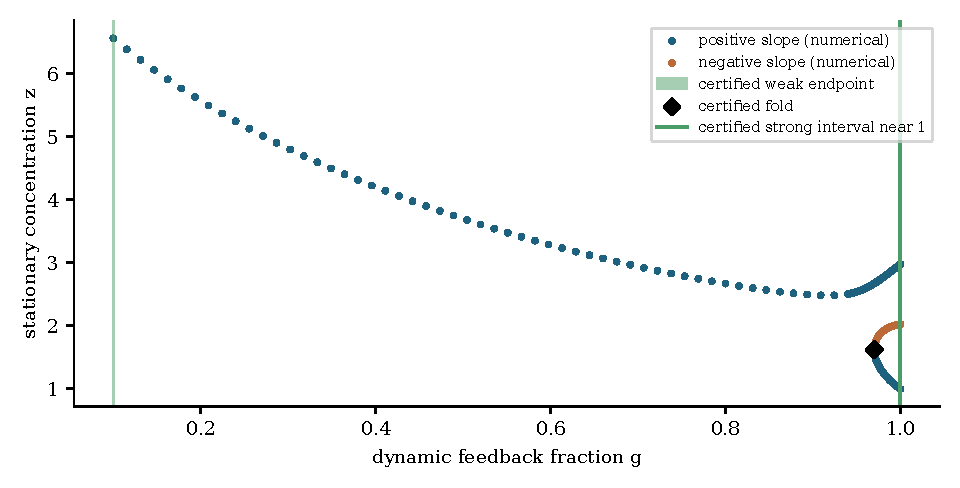
\includegraphics[width=.92\linewidth]{figures/feedback.pdf}
\caption{Stationary response of the routed family at $e=10^{-5}$ as the dynamic feedback fraction $g$ varies. Dots are numerical roots of $Q_e(\cdot,g)$ with positive reconstruction, coloured by the numerical sign of $\partial_zQ_e$; they are an illustration, not a certified bifurcation diagram. Certified elements: the weak endpoint $g=0.1$ (one state), the strong interval $g\in(0.999999,1)$ (two attracting states, Theorem~\ref{thm:C}; too narrow to resolve at this scale), and the rationally isolated fold (diamond, Theorem~\ref{thm:fold}).}\label{fig:feedback}
\end{figure}

\section{Global convergence and state selection: the flagship family}\label{sec:global}

\subsection{Positivity, continuation, and an absorbing region}

\begin{lemma}\label{lem:absorbing}
Let $e\in I$. Positive solutions of~\eqref{eq:ode} remain positive and exist for all forward time, and every positive solution enters in finite time and thereafter remains in the compact forward-invariant set
\begin{equation}\label{eq:Omega}
\Omega=\Bigl\{A,B,z,H\ge0:\ A+B\le34,\ z+\tfrac74H\le384,\ z\le12,\ B\ge2\Bigr\}.
\end{equation}
In particular $0\le A\le34$, $2\le B\le34$, $0\le z\le12$ and $0\le H\le1536/7$ on $\Omega$.
\end{lemma}
\begin{proof}
On each coordinate face the field is inward or tangent: $\dot A=6+Bz+2eB>0$ at $A=0$, $\dot B=27+A+eA^2>0$ at $B=0$, $\dot z=A+3H\ge0$ at $z=0$ and $\dot H=16z+2z^2\ge0$ at $H=0$; a first-crossing argument preserves strict positivity. Let $S=A+B$ and $W_1=z+\tfrac74H$. From~\eqref{eq:ode}, $\dot S=33-S+eB-eA^2\le33-(1-e)S$, and while $S\le34$,
\[
\dot W_1=A-Bz+12z-\tfrac12z^2-\bigl(\tfrac12+\tfrac74d\bigr)H\le\tfrac{5364}{49}-\tfrac27W_1 ,
\]
using $A\le34$ and $\max_z(\tfrac{82}{7}z-\tfrac12z^2)=6724/98$. These differential inequalities bound the solution on every finite interval, excluding blow-up, and comparison gives persistent $S\le34$ and then $W_1\le384$ after finite times. In those half-spaces, $z\ge12$ implies $\dot z\le34-192-576+3\cdot\tfrac47(384-12)=-674/7$, and $B\le2$ implies $\dot B\ge27-26-2e\ge24999/25000$. Hence every positive trajectory enters $\Omega$ in finite time, and each face inequality persists by first crossing.
\end{proof}

\subsection{The response potential}

Put $q(B)=33-B+eB$ and define the response branch
\begin{equation}\label{eq:responses}
a_h(B)=\frac{2q(B)}{1+\sqrt{1+4eq(B)}},\qquad h(B)=B+a_h(B),\qquad c(B)=h'(B)=\frac{e(1+2a_h(B))}{1+2ea_h(B)} .
\end{equation}
$a_h(B)$ is the unique $A$ solving the second balance $eA^2+A+(1-e)B=33$ of~\eqref{eq:balance} for given $B$; equivalently $h+e(h-B)^2=33+eB$. On $2\le B\le34$ one has $-1\le a_h\le33$ and $|c|\le1/500$. Define the residuals
\begin{equation}\label{eq:residuals}
\begin{gathered}
r=A+B-h(B),\qquad \alpha=1+e\bigl(A+a_h(B)\bigr),\qquad F_1=60-(2+z)B,\\
Z=h(B)-(1+z)B-16z-4z^2+3H,\qquad K=16z+2z^2-(2+d)H .
\end{gathered}
\end{equation}
Then~\eqref{eq:ode} is exactly
\begin{equation}\label{eq:residual-ode}
\dot B=F_1+\alpha r,\qquad \dot z=Z+r,\qquad \dot H=K,\qquad \dot r=-\alpha(1+c)r-cF_1 ,
\end{equation}
so that $(B,z,H,r)$ are coordinates on $D$ and the stationary states are exactly the common zeros of $(r,F_1,Z,K)$. The set $r=0$ is not invariant. With
\[
L(z)=\log\frac{z+1}{z+2},\qquad \beta(B)=\frac{60}{B}-2,\qquad \varphi(H)=\frac{2(2+d)H}{16+\sqrt{256+8(2+d)H}}
\]
(so that $16\varphi+2\varphi^2=(2+d)H$, i.e.\ $\varphi(H)$ is the $z$ value at which $K=0$), and the definite primitives
\begin{equation}\label{eq:primitives}
\begin{gathered}
U(z)=\int_0^z\frac{16v+4v^2}{(v+1)(v+2)}\dd v,\qquad
R(H)=\int_0^H3L(\varphi(v))\dd v,\\
P(B)=\int_{20}^B\Bigl[\log\frac v{60}+c(v)\log\Bigl(1-\frac v{60}\Bigr)\Bigr]\dd v,
\end{gathered}
\end{equation}
the \emph{response potential} is
\begin{equation}\label{eq:V}
\boxed{\;V(A,B,z,H)=B\log(2+z)-h(B)L(z)+U(z)-3HL(z)+P(B)+R(H)+\tfrac12r^2 .\;}
\end{equation}
All radicals and logarithms are admissible on a neighbourhood of $\Omega$. $V$ is not a Lyapunov function in the sense of being minimized at a single equilibrium; it is a function that strictly decreases along every nonstationary trajectory in $\Omega$, and its role is exactly that.

\begin{lemma}[Strict response dissipation]\label{lem:diss}
Along every solution in $\Omega$,
\begin{equation}\label{eq:diss}
\dot V\le-\D,\qquad \D=\frac{r^2}4+\frac{F_1^2}{1000}+\frac{Z^2}{364}+\frac{K^2}{4000},
\end{equation}
and $\D=0$ exactly at the stationary points.
\end{lemma}
\begin{proof}
Write $V_0=V-\tfrac12r^2$, a function of $(B,z,H)$ only, and $w=(z+1)(z+2)$. Differentiating~\eqref{eq:V},
\[
\partial_BV_0=\log\frac{B(2+z)}{60}-c\bigl[L(z)-L(\beta(B))\bigr],\qquad
\partial_zV_0=-\frac Zw,\qquad
\partial_HV_0=3\bigl[L(\varphi(H))-L(z)\bigr].
\]
Since $(2+\beta)B=60$, the first expression equals $\Psi(z)-\Psi(\beta)$ with $\Psi(\zeta)=\log(2+\zeta)-cL(\zeta)$ and $\Psi'(\zeta)=(1-c/(1+\zeta))/(2+\zeta)$. The mean value theorem and $z-\beta=-F_1/B$ give $\partial_BV_0=-mF_1$ with $m=\Psi'(\xi)/B$ for some $\xi$ between $z$ and $\beta$; there $1+\xi\ge13/17$ and $B(2+\xi)$ lies between $60$ and $B(2+z)\in[4,476]$, so $1/500\le m\le13/50$. Next, $\partial_HV_0\,K=-3L'(\zeta)\,\psi'(\zeta')\,(z-\varphi)^2$ with $\psi(z)=16z+2z^2$, and $K=\psi'(\zeta')(z-\varphi)$; since $0\le\varphi<12$, $L'\ge1/182$ and $\psi'\le64$ on $[0,12]$, we get $\partial_HV_0\,K\le-K^2/4000$. Substituting~\eqref{eq:residual-ode},
\[
\dot V\le-mF_1^2-\frac{Z^2}w-\frac{K^2}{4000}-\alpha(1+c)r^2-(\alpha m+c)\,rF_1-\frac{rZ}w .
\]
Bound $|\alpha mrF_1|\le\tfrac m4F_1^2+\alpha^2mr^2$, $|crF_1|\le\tfrac m4F_1^2+(c^2/m)r^2$ and $|rZ|/w\le(Z^2+r^2)/(2w)$. With $99/100\le\alpha\le101/100$ and $2\le w\le182$, the remaining coefficient of $r^2$ is at least
\[
\frac{99}{100}\cdot\frac{499}{500}-\Bigl(\frac{101}{100}\Bigr)^2\frac{13}{50}-\frac{(1/500)^2}{1/500}-\frac14=\frac{235397}{500000}>\frac14 ,
\]
the coefficient of $F_1^2$ is at least $m/2\ge1/1000$, and that of $Z^2$ is at least $1/(2w)\ge1/364$. This is~\eqref{eq:diss}. By~\eqref{eq:residual-ode}, $\D=0$ if and only if the full field vanishes.
\end{proof}

\subsection{Convergence of every trajectory}

\begin{proof}[Proof of Theorem~\ref{thm:G}, convergence part]
By Lemma~\ref{lem:absorbing} every positive solution eventually lies in $\Omega$, where $V$ is bounded below and, by Lemma~\ref{lem:diss}, nonincreasing; hence $\int^\infty\D(X(t))\dd t<\infty$. The field and the derivatives of $\D$ are bounded on $\Omega$, so $t\mapsto\D(X(t))$ is uniformly continuous, and integrability forces $\D(X(t))\to0$. Every $\omega$-limit point is therefore stationary (this is LaSalle's principle~\cite{lasalle1960} with the strict dissipation making the invariant set equal to the stationary set). A stationary point of $\Omega$ is positive: $A=0$ contradicts $\dot A>0$ there, $B\ge2$ on $\Omega$, $z=0$ forces $H=0$ from $\dot H=0$ and then $\dot z=A>0$, and $H=0$ contradicts $z>0$. By Theorem~\ref{thm:count} the $\omega$-limit set is contained in $\{s_-,s_0,s_+\}$; being connected, it is a single point. Thus every positive solution converges; polynomial local uniqueness identifies every forward solution with the one obtained by continuation.
\end{proof}

\subsection{The barrier, the energy ordering, and the selection rule}

\begin{proposition}[Plane barrier and energy ordering]\label{prop:barrier}
For $x\in\Omega$ with $B(x)=B(s_0)$ one has $V(x)\ge V(s_0)$. Moreover
\begin{equation}\label{eq:well}
V(s_-)<V(s_0),\qquad V(s_+)<V(s_0),\qquad B(s_-)>B(s_0)>B(s_+).
\end{equation}
\end{proposition}
\begin{proof}
Fix $B$ and $z$. As a function of $H$, $\partial_HV_0=3[L(\varphi(H))-L(z)]$ is increasing (both $L$ and $\varphi$ increase) and vanishes exactly at $H^*(z)=(16z+2z^2)/(2+d)$, so $V_0(B,z,\cdot)$ is minimized at $H^*(z)$. On the section $H=H^*(z)$ the $z$ derivative of $V_0(B,z,H^*(z))$ equals $\partial_zV_0=-Z/w$ with $H=H^*(z)$, that is
\[
\frac{(1+z)B-h(B)+k(z)}{(1+z)(2+z)} ,
\]
whose numerator has $z$-derivative $B+k'(z)>0$ whenever $B\ge8$, because $k'(z)>-8$. On the plane $B=B(s_0)\ge8$ this numerator is strictly increasing and vanishes at $z(s_0)$ (where $Z=0$), so $z(s_0)$ is the unique minimizer. Since $V=V_0+\tfrac12r^2\ge V_0$ and $r(s_0)=0$, every $x\in\Omega$ with $B(x)=B(s_0)$ satisfies $V(x)\ge V_0(B(s_0),z(x),H^*(z(x)))\ge V_0(s_0)=V(s_0)$.

For~\eqref{eq:well}, restrict $V$ to the response curve $\gamma(z)=(A_g(z),60/(2+z),z,H^*(z))$ at $g=1$, on which $r=0$, $F_1=0$ and $K=0$. Then $\frac{\dd}{\dd z}V(\gamma(z))=\partial_BV_0\cdot B'(z)+\partial_zV_0=-Z/w$, since $\partial_BV_0=-mF_1=0$ on the curve. On the curve $Z=a_h(B)-A_g(z)$, and because $\xi\mapsto e\xi^2+\xi$ is increasing, $A_g-a_h$ has the sign of $eA_g^2+A_g-(ea_h^2+a_h)=Q_e(z,1)$. Thus $V\circ\gamma$ increases where $Q_e>0$, namely on $(z_-,z_0)$, and decreases where $Q_e<0$, namely on $(z_0,z_+)$ (Theorem~\ref{thm:count}); hence $V(s_\pm)<V(s_0)$. Finally $B=60/(2+z)$ is decreasing in $z$.
\end{proof}

\begin{proof}[Proof of Theorem~\ref{thm:G}, selection rule]
Let $x\in\Omega$ with $V(x)<V(s_0)$ and $B(x)>B(s_0)$. Along the trajectory $V$ is nonincreasing, so $V<V(s_0)$ for all later times, and by Proposition~\ref{prop:barrier} the plane $B=B(s_0)$ can never be reached; by continuity $B>B(s_0)$ forever. The limit is an equilibrium with $V\le V(x)<V(s_0)$ and $B\ge B(s_0)$, which excludes $s_0$ and, by~\eqref{eq:well}, $s_+$. Hence $x\in\B_{s_-}$. The case $B(x)<B(s_0)$ is symmetric. Small perturbations of $s_\pm$ satisfy the respective strict inequalities, so both selected sets contain open neighbourhoods of the sinks, and the basins are nonempty.
\end{proof}

\subsection{Saddle geometry: local invariant graphs, branch destinations, and the basin boundary}\label{sec:geometry}

Let $s_0$ be the middle equilibrium. By Theorem~\ref{thm:count} its Jacobian has three real eigenvalues below $-1/2$ and one real eigenvalue $\lambda\in(0,1/10)$. In physical eigen-coordinates $(v,u)\in\R^3\times\R$ near $s_0$,
\[
\dot v=Sv+N_s(v,u),\qquad \dot u=\lambda u+N_u(v,u),\qquad \max\sigma(S)<-\tfrac12,\ \lambda>0,
\]
with $N=(N_s,N_u)$ quadratic and $DN(0)=0$.

\emph{Local stable graph and local coverage.} For a small stable coordinate $v_0$ the integral equations
\[
v(t)=e^{St}v_0+\int_0^te^{S(t-\tau)}N_s(v,u)(\tau)\dd\tau,\qquad
u(t)=-\int_t^\infty e^{\lambda(t-\tau)}N_u(v,u)(\tau)\dd\tau
\]
define a contraction on a small ball of an exponentially weighted space, with a weight strictly between $0$ and the smallest decay rate~\cite[Section~2.7]{perko2001}. The fixed point depends analytically on $v_0$ because the nonlinear map is analytic with derivative of norm less than one. The initial states form an analytic graph $u=\gamma(v)$ with $\gamma(0)=0$, $D\gamma(0)=0$, and every solution that stays in the small ball for all positive times satisfies the same integral equations (the growing homogeneous term must vanish) and therefore lies on the graph. Reversing time gives the analytic local unstable curve, whose backward trajectories converge to $s_0$.

\emph{Branch destinations.} The $B$ component $b$ of the unstable eigenvector is nonzero: if it vanished, adding the first two eigenvector equations of~\eqref{eq:J} would give $(\lambda+1+2eA_0)a=0$, hence $a=0$, and the second and third rows would force the remaining components to vanish. A nonstationary unstable-branch trajectory has $V<V(s_0)$ (integrate the strict dissipation from any finite past time and use the backward limit), and for a small curve parameter $u$ its $B$ side is the sign of $ub$. By the selection rule the branch with $ub>0$ converges to $s_-$ and the branch with $ub<0$ to $s_+$; both branches lie in $D$ since $D$ is forward invariant and the branches start in $\Omega$.

\begin{lemma}[Annular energy cost]\label{lem:annulus}
Suppose a trajectory crosses from the ball of radius $\rho/2$ about an equilibrium to the sphere of radius $\rho$, staying in a region where its speed is at most $M>0$, $V$ is nonincreasing, and $\D\ge d_\rho>0$ on the annulus $\rho/2\le\dist\le\rho$. Then the crossing costs at least $c_\rho=d_\rho\rho/(2M)$ in $V$.
\end{lemma}
\begin{proof}
Let $\tau$ be the first exit time from the radius-$\rho$ ball. Covering the radial distance $\rho/2$ takes at least $\rho/(2M)$ time; during the last $\rho/(2M)$ before $\tau$ the distance is at least $\rho/2$ by the speed bound and at most $\rho$ by first exit. Integrating~\eqref{eq:diss} over that window gives the claim.
\end{proof}

\emph{No return: the local middle basin is the stable graph.} Choose an annulus about $s_0$ inside the interior of $\Omega$ and away from $s_\pm$; compactness and Lemma~\ref{lem:diss} give $d_\rho>0$, and the field supplies $M$. A trajectory tending to $s_0$ has $V\ge V(s_0)$ at all times. Starting sufficiently close to $s_0$ makes $V(X(0))-V(s_0)<c_\rho$, so by Lemma~\ref{lem:annulus} such a trajectory can never leave the radius-$\rho$ ball, hence lies on the local stable graph. Conversely every point of the graph tends to $s_0$. Thus, for every small radius, the middle basin near $s_0$ is exactly the graph, not merely a trapped subset of it.

\emph{Global analytic hypersurface.} Every $x\in W=\B_{s_0}$ reaches the local neighbourhood at a finite time $T$. The time-$T$ map $\Phi_T$ is analytic and locally invertible near $x$: solve the polynomial equation on a compact tube about the finite orbit segment and the reversed equation on the reversed segment; only finite backward existence is used. The analytic shear $(v,u)\mapsto(v,u-\gamma(v))$ straightens the local graph. Composing it with $\Phi_T$ gives analytic ambient coordinates at $x$ in which $W$ is exactly the coordinate plane $\{w=0\}$. Hence $W$ is an embedded real-analytic hypersurface of $D$.

\emph{Basin boundary.} In straightened coordinates near $s_0$ the transverse coordinate obeys $\dot u=(\lambda+O(\rho))u$ in a small box. As a nonzero initial transverse displacement tends to zero, its exit time tends to infinity and, by variation of constants in the stable coordinates, its exit point approaches the exit point of the corresponding unstable branch, which lies in the open basin of a sink. Hence arbitrarily small displacements of either sign select opposite sinks, and transporting this back by the finite-time inverse shows that every point of $W$ is a boundary point of both $\B_{s_-}$ and $\B_{s_+}$. Conversely a boundary point of a sink basin inside $D$ belongs to neither open sink basin, and since every positive trajectory converges to one of $s_-,s_0,s_+$, it lies in $W$. This proves~\eqref{eq:boundary} and completes the proof of Theorem~\ref{thm:G}.

\subsection{Consequences: measure, an eventual test, and a dissipation budget}\label{sec:consequences}

\begin{corollary}\label{cor:null}
$\Leb_4(W)=0$ and $D\setminus W=\B_{s_-}\,\dot\cup\,\B_{s_+}$. Every probability distribution on $D$ that is absolutely continuous with respect to Lebesgue measure selects a sink with probability one.
\end{corollary}
\begin{proof}
$W$ is second countable, so the cover by the ambient chart neighbourhoods of Section~\ref{sec:geometry} has a countable subcover. In each chart $W$ is the plane $\{w=0\}$, which is null by Fubini; exhausting the chart target by countably many compact balls on which the analytic inverse is Lipschitz, and using that Lipschitz maps preserve null sets, each chart piece of $W$ is null, and so is the countable union. The disjoint decomposition follows from global convergence and uniqueness of limits.
\end{proof}

The distinction between the two open basins is retained in the final composition even though, by Theorem~\ref{thm:A}, the eventual activity labels agree. This concerns uncertainty in deterministic initial conditions only.

\begin{proposition}[Eventual completeness of the selection test]\label{prop:decision}
Every trajectory in $\B_{s_-}$ eventually satisfies, for all later times, $X(t)\in\Omega$, $V(X(t))<V(s_0)$ and $B(X(t))>B(s_0)$; every trajectory in $\B_{s_+}$ eventually satisfies the same energy test with $B(X(t))<B(s_0)$.
\end{proposition}
\begin{proof}
$\Omega$ is eventually invariant by Lemma~\ref{lem:absorbing}; the strict inequalities~\eqref{eq:well} persist in a neighbourhood of the limit. Take the maximum of the three entry times.
\end{proof}

\begin{remark}[What one computes along a trajectory]\label{rem:test}
The test is: after entry into $\Omega$, evaluate $V(X(t))$ by~\eqref{eq:V} and compare it with $V(s_0)$, and compare $B(X(t))$ with $B(s_0)$. If both strict inequalities hold at any single time, the eventual state is certified (Theorem~\ref{thm:G}); by Proposition~\ref{prop:decision} the test eventually succeeds for every trajectory off $W$. It is a decision from the trajectory after a transient, not from the initial state alone, and no uniform decision time is claimed near $W$. For computable $e\in I$ and computable initial data the test is semidecidable: the three simple roots have rational brackets; the radicals, logarithms and definite integrals of~\eqref{eq:V} are computable with certified error on compact interior boxes; and validated finite-time enclosures of the polynomial flow (interval Taylor or Picard bounds) at increasing times and precisions terminate off $W$, since each equilibrium is strictly inside every face of $\Omega$ and the limiting inequalities are strict. The illustrations below are not an implementation of this verifier; a numerically observed verdict is not a rigorously enclosed one. The heuristic ``choose the nearer equilibrium'' is not what is proved.
\end{remark}

\begin{proposition}[Integrated dissipation and residence]\label{prop:budget}
Let $t_0$ be a time after which $X(t)\in\Omega$ and let $s_\infty$ be the limit. Then $\int_{t_0}^\infty\D(X(t))\dd t\le V(X(t_0))-V(s_\infty)=:\Delta V$. For $\delta>0$ let $C_\delta=\{x\in\Omega:\dist(x,\{s_-,s_0,s_+\})\ge\delta\}$; if $C_\delta\ne\varnothing$ then $d_\delta=\min_{C_\delta}\D>0$ and
\[
\Leb_1\{t\ge t_0:\dist(X(t),\{s_-,s_0,s_+\})\ge\delta\}\le\Delta V/d_\delta .
\]
For $N$ disjoint completed annular crossings after $t_0$, each costing at least $c>0$ as in Lemma~\ref{lem:annulus}, $Nc\le\Delta V$.
\end{proposition}
\begin{proof}
Integrate~\eqref{eq:diss} to $T$ and let $T\to\infty$ using monotone convergence and $V(X(T))\to V(s_\infty)$. Compactness gives the attained minimum on $C_\delta$, which contains no stationary point. Integrate $d_\delta$ times the indicator of the residence set. Crossing losses on disjoint windows add, since $V$ never increases.
\end{proof}

These bound the time spent away from all three equilibria and the number of completed excursions; they do not bound the time spent near $s_0$ and therefore give no uniform time to the selected sink.

\begin{figure}[!tbp]\centering
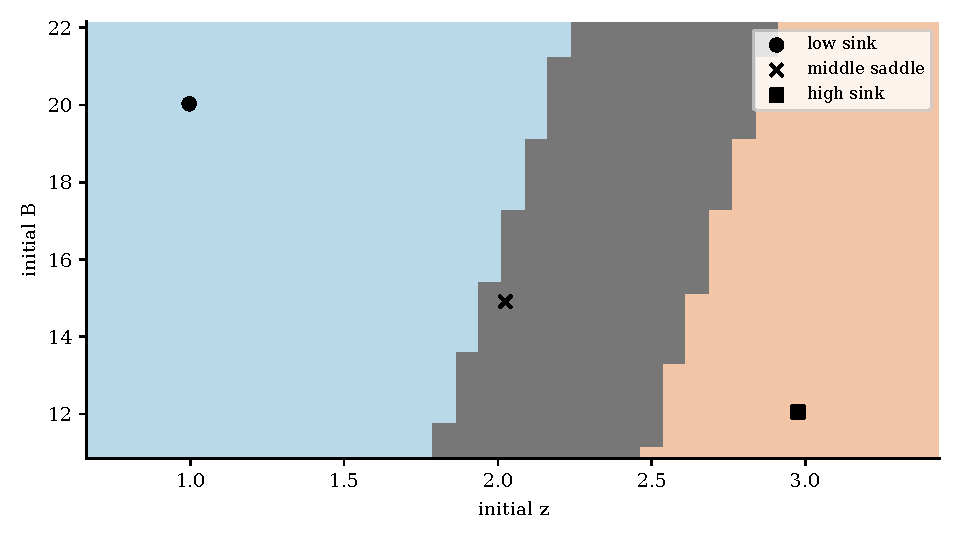
\includegraphics[width=.9\linewidth]{figures/basins.pdf}
\caption{Illustrative finite-time basin slice at $e=10^{-5}$, $g=1$. The plotted coordinates are the initial $z$ and $B$; the remaining initial coordinates are fixed by $A=h(B)-B$ (so $r=0$) and $H=H^*(z)$, a curved two-dimensional surface containing all three equilibria. A $37\times37$ grid is integrated numerically to $T=400$. Blue and orange mark numerical proximity within $0.02$ (maximum norm) to $s_-$ and $s_+$; dark grey marks cells unresolved at this horizon ($337$ of $1369$). This is a slice, not a projection, and the coloured boundary is not the four-dimensional separator $W$; no global $B$ threshold is inferred.}\label{fig:basin}
\end{figure}

\begin{figure}[!tbp]\centering
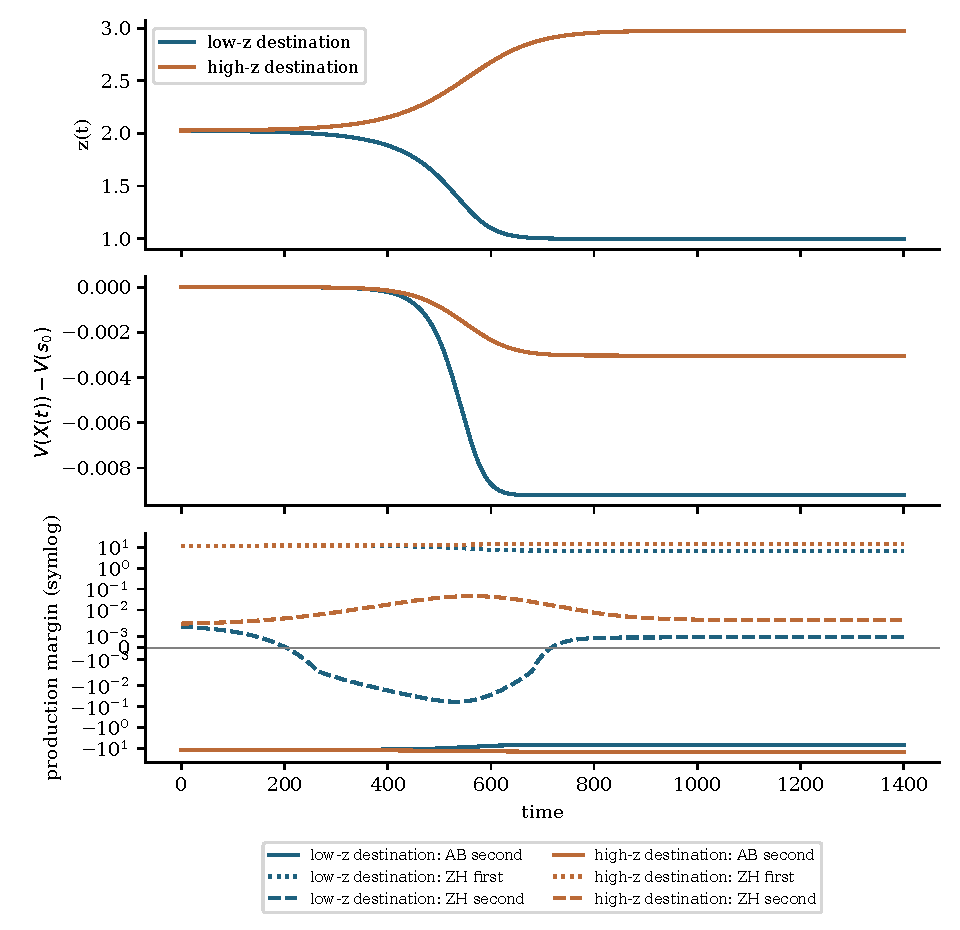
\includegraphics[width=.8\linewidth]{figures/traces.pdf}
\caption{Numerical traces from $s_0\pm0.02\,v_u$, where $v_u$ is the unit unstable eigenvector oriented with positive $B$ component, at $e=10^{-5}$, $g=1$ (Radau, relative tolerance $2\cdot10^{-10}$). Top: the $z$ concentration separates the destinations. Middle: $V(X(t))-V(s_0)$, computed from~\eqref{eq:V} by quadrature, decreases and settles below zero on both sides, as the selection test requires. Bottom (symmetric log scale): the $\cAB$ production $p_{AB,B}$ stays negative while both $\cZH$ productions become and remain positive, so the two destinations share the eventual signature of Theorem~\ref{thm:A}. These integrations illustrate the proved statements and are not validated enclosures; the initial states are close to, but not on, $W$.}\label{fig:traces}
\end{figure}

\section{Activity along trajectories and what the signature cannot see}\label{sec:activity}

\begin{proof}[Proof of Theorem~\ref{thm:A}]
At a stationary state~\eqref{eq:ode} gives $p_{AB,B}=j-k=B-27$ (from $\dot B=0$), $p_{ZH,H}=\ell-m=dH$ (from $\dot H=0$), and $p_{ZH,z}=-\ell+2m=-j=-k(z)$ (from $\dot z=0$ and the third balance of~\eqref{eq:balance}). By Theorem~\ref{thm:count} every positive equilibrium has $z\in(0.9,3.1)$, hence $B=60/(z+2)<60/2.9<21$, so $p_{AB,B}<-6$; $-k(z)>6.3$ on the three brackets, so $p_{ZH,z}>4$; and $H=(16z+2z^2)/(2+d)>8$, so $p_{ZH,H}>1/2000$. In particular $\cZH$ is strictly productive and $\cAB$ is not at each equilibrium. Every positive solution converges to an equilibrium (Theorem~\ref{thm:G}) and the production functions are continuous, so the strict margins~\eqref{eq:margins} hold for all large $t$ with half the stationary slack. The two sinks have distinct $z$, hence distinct $B=60/(z+2)$, $A=zB+k(z)$ and $H$.

For the transient bound, $p_{AB,A}\ge\eta$ and $p_{AB,B}\ge\eta$ give $k\ge2\eta$ and $j\ge3\eta$, and then $\dot z=j+p_{ZH,z}\ge4\eta$ by~\eqref{eq:balance-identity} (whose right side is $\dot z$ and whose middle term is $2p_{AB,B}$, so $\dot z=p_{AB,A}+2p_{AB,B}+p_{ZH,z}\ge\eta+2\eta+\eta=4\eta$). Integrating, $4\eta(b-a)\le z(b)-z(a)<12$, hence $b-a\le3/\eta$.
\end{proof}

Table~\ref{tab:compositions} makes the information limit concrete at $e=10^{-5}$. The signature of each equilibrium is the same; the compositions differ in every coordinate, and so do the sizes of the production margins. Agreement of the signature is a consequence of the stationary identities $p_{AB,B}=B-27<0$ and $p_{ZH,H}=dH>0$ together with the bracket bounds; it does not assert equality of fluxes, of production rates, or of any other dynamical property of the two sinks.

\begin{table}[tb]\centering\footnotesize\setlength{\tabcolsep}{4.5pt}
\begin{tabular}{@{}lcccccccc@{}}\toprule
Equilibrium & $A$ & $B$ & $z$ & $H$ & $p_{AB,B}$ & $p_{ZH,z}$ & $p_{ZH,H}$ & signature ($\cAB$, $\cZH$)\\\midrule
$s_-$ (sink) & $12.9704$ & $20.0281$ & $0.99579$ & $8.9575$ & $-6.972$ & $6.973$ & $0.000896$ & (inactive, productive)\\
$s_0$ (saddle) & $18.0895$ & $14.9074$ & $2.02484$ & $20.2977$ & $-12.093$ & $12.096$ & $0.002030$ & (inactive, productive)\\
$s_+$ (sink) & $20.9387$ & $12.0570$ & $2.97637$ & $32.6681$ & $-14.943$ & $14.947$ & $0.003267$ & (inactive, productive)\\\bottomrule
\end{tabular}
\caption{Equilibrium compositions and actual production margins at $e=10^{-5}$, $g=1$. Values are rounded from rational enclosures obtained by exact bisection of~\eqref{eq:P} to width below $10^{-12}$ followed by exact reconstruction (\texttt{data/spectral\_and\_table\_check.json}). The three states carry the same signature and differ in every concentration.}\label{tab:compositions}
\end{table}

\section{Local robustness and a reversible replacement of the sink}\label{sec:persistence}

\begin{proposition}\label{prop:persist}
Fix $e\in I$. Under sufficiently small admissible variations of the six rate coefficients, the two sinks of~\eqref{eq:ode} continue to two distinct positive locally asymptotically stable equilibria whose strict actual-current activity margins persist, and nearby attracted trajectories eventually have the same signature. In particular the reversible sink $H\rightleftharpoons W_H$ with outgoing coefficient $d$ and incoming buffered flux $\eta>0$, which replaces $\dot H$ by $\dot H+\eta$, has two such equilibria for every sufficiently small $\eta>0$, and admits a common finite-potential thermodynamic realization with an independently adjustable waste potential.
\end{proposition}
\begin{proof}
Each sink has an invertible stationary Jacobian (Theorem~\ref{thm:count}). The implicit function theorem continues it uniquely in a small positive neighbourhood for all nearby parameters; intersect the two parameter neighbourhoods and choose disjoint state neighbourhoods. Continuity of the characteristic roots preserves strictly negative real parts; explicitly, the Lyapunov solution $P=\int_0^\infty e^{J^{\mathsf T}t}e^{Jt}\dd t$ of $J^{\mathsf T}P+PJ=-I$ at the unperturbed sink is positive definite, the quadratic form remains strictly decreasing for nearby Jacobians, and the quadratic remainder is dominated in a small neighbourhood. Strict production inequalities persist by continuity of the currents at the continued equilibria. For the reversible sink, exactness of the reconstruction survives: with $\ep=\eta$ the stationary state has $B_{p,\ep}=B_p$, $H_{p,\ep}=H_p+\ep/(2+d)$, $A_{p,\ep}=A_p-3\ep/(2+d)$ and residual $E_{p,\ep}=b-(1+e)B_p+K_p-3\ep/(2+d)+e(A_p-3\ep/(2+d))^2$, depending smoothly on $\ep$, so the continuation applies; at a stationary point $p_{ZH,H}=dH_{p,\ep}-\ep$, and activity is preserved by a strict inequality, not by setting $\ep=0$. For the thermodynamic realization set
\[
\mu_{W_H}=\mu_H-\log\frac d\eta=\log\frac{\eta}{2d} ,
\]
so that $d/\eta=\exp(\mu_H-\mu_{W_H})$ while every other relation in~\eqref{eq:mu} is unchanged because $W_H$ appears in no other reaction; the equal masses of $H$ and $W_H$ preserve mass balance. This is a separate verification, not a consequence of smallness of $\eta$: if $\mu_{W_H}$ were held at zero the ratio would force $\eta=2d$. The limit $\eta\downarrow0$ sends the waste potential to $-\infty$, so the ideal sink is not a small perturbation in all thermodynamic potentials.
\end{proof}

The same hyperbolic persistence applies at each routed attracting state of Theorem~\ref{thm:C}. None of these local statements extends the global convergence theorem, the exact equilibrium count, or the basin geometry to the perturbed families; numerical checks at $\eta=10^{-6}$ and $10^{-4}$ (\texttt{data/figure\_summary.json}) illustrate persistence but certify no uniform interval of reverse inputs.

\section{Discussion}\label{sec:discussion}

\emph{What the intervention shows.} Each module alone, with its reservoirs and loads retained, has one response to any fixed environment (Proposition~\ref{prop:clamped}); the decoupled assembly and every weakly coupled assembly have one stationary state (Proposition~\ref{prop:weak}). Re-routing the fork so that its product $z$ becomes a dynamic variable seen by the other module, at fixed total capacity, creates a second attracting composition (Theorem~\ref{thm:C}) through a nondegenerate saddle-node (Theorem~\ref{thm:fold}). The mechanism is a decreasing load secant (Lemma~\ref{lem:load}): two compatible balances require the load $k$ to decrease between their $z$ values, which is possible only because, for $d<1$, the load carries the negative term $-u(1-d)z/(2+d)$. This is a statement about this assembly; it is not a criterion for arbitrary coupled cores.

\emph{What determines the selected composition.} In the flagship family the answer is exact: the initial state lies on one side of the analytic separator $W$ or the other, and outside a null set this is decided by the eventual energy-and-side test of Proposition~\ref{prop:decision}. The potential $V$ is not minimized at a single state; it is a strictly dissipated function whose value at the saddle is a barrier on the plane $B=B(s_0)$. Convergence is not uniform in time, no rate is claimed, and the residence bounds of Proposition~\ref{prop:budget} do not bound time near the saddle.

\emph{What the activity signature misses.} The eventual signature ($\cAB$ inactive, $\cZH$ productive) is the same at both sinks and indeed at all three equilibria; the selected composition is invisible to it, though visible in every concentration and in the sizes of the production margins (Table~\ref{tab:compositions}). For a reactor whose state is later read out only through core activities, this is a loss of information about the initial condition; for a reactor whose composition is read out, the two sinks are two distinguishable chemical states. Whether such a state can be copied reliably through growth, division and recovery under molecular noise is a different question, addressed for a related construction in~\cite{copying2026}; nothing here establishes inheritance.

\emph{Limitations.} The global theorems hold on the flagship interval $I$ with the ideal sink; the routed theorems hold on $\Rr$ and on the certified fold box; we do not classify the whole routed family, assert uniqueness of the fold, extend global convergence to the reversible-sink extension, or claim any experimental validation. The two distinguished cores are not claimed to exhaust the autocatalytic cores of the network. The figures are illustrations.

\appendix

\section{Finite certificates}\label{app:cert}

\emph{Descartes count.} Table~\ref{tab:descartes} lists the integer coefficients of $\widetilde P_e(t)=\sum_i(C_i+D_ie)t^i$ from the proof of Theorem~\ref{thm:count}. Substitution of $e=1/200000$ and $e=1/50000$ gives the indicated strict signs; affine dependence on $e$ makes them persist on $I$.

\begin{table}[htb]\centering\small
\begin{tabular}{@{}rrrc@{}}\toprule
$i$ & $C_i$ & $D_i$ & sign on $I$\\\midrule
0 & $-533386668$ & $-5333866680$ & $-$\\
1 & $2490844536$ & $-53338666800$ & $+$\\
2 & $17625654572$ & $5321310601944$ & $+$\\
3 & $-56063923056$ & $9698165540064$ & $-$\\
4 & $-58946493844$ & $19289023400056$ & $-$\\
5 & $105146857080$ & $13527216754000$ & $+$\\
6 & $93428004500$ & $10222548740200$ & $+$\\\bottomrule
\end{tabular}
\caption{Exact coefficients of the transformed stationary polynomial; three sign changes.}\label{tab:descartes}
\end{table}

\emph{Bernstein sign tests.} The identity $b_k=\sum_{j=0}^ka_j\binom kj/\binom nj$ converts power coefficients on $[0,1]$ into Bernstein coefficients of degree $n$; positivity of all $b_k$ bounds the polynomial below by $\min_kb_k$ on the whole interval. The spectral tests in Theorem~\ref{thm:count} use $n=3$ in $z$ after the affine map of each bracket onto $[0,1]$, and affine dependence on $(e,q)$ reduces them to the four corners. The derivative bounds used in the alternative route are $P_e''(0)\in[-87557130,-84975256]$ and $P_e^{(4)}([0,12])\subset[1052234744,1115677376]$ by direct interval evaluation. The routed root signs in the proof of Theorem~\ref{thm:C} use the numerator of $Q_e$ at the four displayed $z$ endpoints, Bernstein conversion of degree four in $g$ on $[999999/10^6,1]$, and the endpoints in $e$. The script \texttt{scripts/check\_spectra\_and\_table.py} recomputes the spectral bounds and Table~\ref{tab:compositions} in exact arithmetic.

\emph{Comparison weights.} Table~\ref{tab:weights} lists the positive rational weights of the certificates of Theorem~\ref{thm:C} and Remark~\ref{rem:cac} (terminating decimals denote exact rationals). For a box with bounds $A_l,A_u,B_l,B_u,z_l,z_u,H_l,H_u$ the comparison matrix is determined without rounding by $M_{11}=-1-2eA_l$, $M_{12}=e(1+2A_u)$, $M_{21}=1+2eA_u$, $M_{22}=-3+g-gz_l-e-2eA_l$, $M_{23}=gB_u$, $M_{31}=g$, $M_{32}=g(1+z_u)$, $M_{33}=-gB_l-16-8z_l$, $M_{34}=3$, $M_{43}=16+4z_u$, $M_{44}=-2-d$, with $g$ replaced by its interval endpoints where the sign requires, and all other entries zero. Direct rational arithmetic verifies $l,r>0$, the four inequalities~\eqref{eq:row} with $\kappa=1/100$, and $1/4\le l_i/r_i\le100$.

\begin{table}[htb]\centering\small
\begin{tabular}{@{}lll@{}}\toprule
 & $l$ & $r$\\\midrule
low box & $(44.8772,\ 17.7482,\ 26.136,\ 39.7021)$ & $(1.0128,\ 48.429,\ 7.1441,\ 71.8776)$\\
high box & $(84.2304,\ 37.0897,\ 46.1605,\ 69.7372)$ & $(1.0138,\ 33.2138,\ 13.5426,\ 189.4476)$\\\bottomrule
\end{tabular}
\caption{Left and right weights of the comparison-energy certificates.}\label{tab:weights}
\end{table}

\begin{table}[htb]\centering\small
\begin{tabular}{@{}llll@{}}\toprule
Branch & Species & Lower bound & Upper bound\\\midrule
low & $A$ & $12.970413$ & $12.970471$\\
low & $B$ & $20.028062$ & $20.02809$\\
low & $z$ & $0.995784$ & $0.995805$\\
low & $H$ & $8.957499$ & $8.95753$\\
high & $A$ & $20.938722$ & $20.938776$\\
high & $B$ & $12.056976$ & $12.056999$\\
high & $z$ & $2.976357$ & $2.976378$\\
high & $H$ & $32.668053$ & $32.668088$\\\bottomrule
\end{tabular}
\caption{Expanded rational state boxes of the flagship certificate at $e=10^{-5}$, $g=1$ (Remark~\ref{rem:cac}); the reconstructed roots lie strictly inside.}\label{tab:cacboxes}
\end{table}

\section{Reproducing the fold certificate}\label{app:fold}

The script \texttt{scripts/certify\_fold.py} implements a closed rational interval class with outward-exact arithmetic on Python fractions. SymPy constructs the rational expressions $Q_e$, $\partial_zQ_e$, their first and second derivatives, and the full physical characteristic polynomial, and differentiates them exactly; no floating-point number enters an acceptance test. The script forms $C=D(Q_e,\partial_zQ_e)(c)^{-1}$ exactly, bounds $I-C\,D(Q_e,\partial_zQ_e)(X)$ in the radius-weighted maximum norm (bound $1.0968\cdot10^{-7}$), and checks that the two components of the centred Newton image lie strictly inside the radii $10^{-9}$ and $10^{-10}$; these two strict checks imply a unique zero by contraction. It then verifies $\partial_gQ_e>0$, $\partial_{zz}Q_e<0$, positive reconstruction, the full-field identity, the determinant identity, and the Hurwitz inequalities of the cubic factor, with the Hurwitz gap $c_1c_2-c_3\in[10297.86359,10297.86362]$. Finally, at $g=1/10$ and $g=1999999/2000000$ an exact Sturm isolation of the cleared polynomial lists respectively one and three positive reconstructed roots, and the gcd of the polynomial with its derivative is one at both endpoints. The output \texttt{data/fold\_certificate.json} records every interval endpoint as an exact fraction; the script \texttt{scripts/check\_principal\_algebra.py} records the endpoint signs and derivative bounds of~\eqref{eq:P} in \texttt{data/principal\_algebra.json}. The numerical labels in Theorem~\ref{thm:fold} are rounded displays of these rational enclosures.

\section{Verification scope and reproducibility}\label{app:verification}

Two Lean~4 developments (toolchain \texttt{leanprover/lean4:v4.30.0}, pinned Mathlib) accompany the paper and were rebuilt with warnings treated as errors while preparing it; both principal declarations depend only on the standard axioms \lean{propext}, \lean{Classical.choice} and \lean{Quot.sound}. The development \lean{CoreCouplingCAC} compiles the literal source adapters, core minimality, clamped uniqueness, unistationarity for $d\ge1$, existence and exact count of the three flagship equilibria with simplicity, the activity balance identity and stationary exclusion, and the quantitative local certificates of Remark~\ref{rem:cac} (principal declaration \lean{coreCouplingCACResolution}). The development \lean{CoreCouplingGlobal} compiles Theorems~\ref{thm:G}, \ref{thm:C} and~\ref{thm:A} through the declaration \lean{phaseTwoResolution}, whose type is the conjunction, over $e\in I$, of the structures \lean{FlagshipGResolution} and \lean{FlagshipAResolution}, together with openness and nonemptiness of \lean{routedBistableRegion}, injectivity of the routed family, and \lean{RoutedCResolution} at every point of that region. Table~\ref{tab:lean} maps the paper's statements to declarations.

\begin{table}[htb]\centering\small
\begin{tabular}{@{}>{\raggedright\arraybackslash}p{.36\linewidth}>{\raggedright\arraybackslash}p{.58\linewidth}@{}}\toprule
Statement & Lean declaration or module\\\midrule
Clamped uniqueness, $d\ge1$ unistationarity & \lean{CoreCouplingCAC.coreCouplingCACResolution}; \lean{Isolation}, \lean{Preservation}, \lean{Existence}\\
Exactly three simple flagship roots & \lean{CoreCouplingCAC.exactly_three_positive_equilibria} (\lean{ExactClassification}, \lean{RootCount}, \lean{RootTransform})\\
Balance identity, stationary exclusion, shared signature & \lean{Activity}: \lean{productivity_balance}, \lean{stationary_core_exclusion}, \lean{selected_same_signature}\\
Quantitative local certificates (Remark~\ref{rem:cac}) & \lean{CoreCouplingCAC.selected_source}, \lean{two_selected_active_equilibria}\\
Every positive trajectory converges & \lean{CoreCouplingGlobal.trajectory_converges_to_positive_equilibrium}\\
Global positive existence & \lean{global_positive_convergent_solution}\\
Basin boundary and analytic charts & \lean{outer_basin_boundaries_equal_middle}; \lean{middle_basin_analytic_manifold_chart}\\
Local stable graph, no return & \lean{SpectralCoverage}, \lean{MiddleNoReturn}, \lean{LocalBasinGraph}\\
Unstable branch destinations & \lean{middle_actual_unstable_branch_destinations}\\
Potential, dissipation, barrier, selector & \lean{ResponsePotential}, \lean{ResidualConvergence}, \lean{WellEnergy}, \lean{NonemptySelector}\\
Routed coexistence (Theorem~\ref{thm:C}) & \lean{core_coupling_C_endpoint}, \lean{routed_C_resolution}\\
Eventual activity (Theorem~\ref{thm:A}) & \lean{flagship_activity_endpoint}, \lean{every_trajectory_eventual_activity}\\
Combined endpoint & \lean{CoreCouplingGlobal.phaseTwoResolution} in \lean{Main.lean}\\\bottomrule
\end{tabular}
\caption{Correspondence between statements and compiled declarations. Unqualified names are in \texttt{CoreCouplingGlobal}.}\label{tab:lean}
\end{table}

The measure-zero, eventual-test and budget results of Section~\ref{sec:consequences}, the fold theorem, and Proposition~\ref{prop:persist} are conventional proofs and are not claimed as Lean declarations. The Lean formalization of Theorem~\ref{thm:C} certifies attraction on the stated boxes; the paper's Lemma~\ref{lem:certificate} is the same argument in conventional form.

The source package accompanying this paper contains the scripts \texttt{certify\_fold.py}, \texttt{check\_principal\_algebra.py}, \texttt{check\_spectra\_and\_table.py}, \texttt{network\_schematic.py} and \texttt{figures.py}, with their JSON, CSV and NPZ outputs. \texttt{figures.py} uses a vectorized fourth-order Runge--Kutta integration for the slice ($\Delta t=0.02$, $T=400$) and an implicit Radau integration for the traces (relative tolerance $2\cdot10^{-10}$, absolute tolerance $2\cdot10^{-12}$), reports unresolved finite-horizon cells rather than assigning them a basin, and evaluates $V$ by quadrature of~\eqref{eq:primitives}; none of its numbers is a proof input.

\bibliographystyle{plain}
\bibliography{refs}

\end{document}
